\documentclass[11pt,a4paper]{report}

\usepackage{datetime}
\usepackage{graphicx}
\usepackage{enumitem}
\usepackage{amsmath}
\usepackage{subcaption}

\usepackage{hyperref}

\hypersetup{
    colorlinks=true,
    linkcolor=blue,
    filecolor=magenta,      
    urlcolor=cyan,
}


\title{Lab Work}
\newdate{date}{28}{06}{2020}
\date{\displaydate{date}}
\author{Nguyen Ngoc Lam}

\begin{document}
  	\pagenumbering{arabic}
  	\tableofcontents
  	\newpage
	
	\chapter{Chapter 1 Lab Work: Overview of Distributed Systems}
	\newpage
	\section{Path of the html File That Contains the Content of the Default Website Apache}
	You can find it at (on linux): /var/www/html/
	\section{Default Port on Which Webserver Is Listening}
	The default port is 80. But you can change it in /etc/apache2/ports.conf (remember to switch to superuser first)
	\begin{figure}[h!]
  		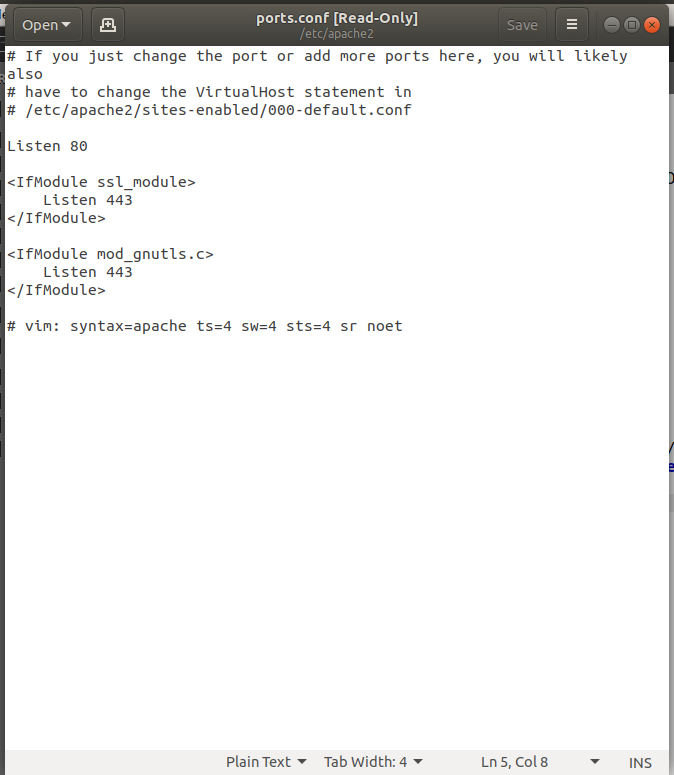
\includegraphics[width=\linewidth]{apache-default-port.png}
  		\caption{Apache port configuration file.}
  		\label{fig:apacheconf}
	\end{figure}
	\newpage
	\section{Meaning of Permission 755}
	\begin{tabular}{|c|c|c|c|}
	\hline 
	• & Write & Execute & Read \\ 
	\hline 
	Value & r & w & x \\ 
	\hline 
	Value (in number) & 4 & 2 & 1 \\ 
	\hline 
	\end{tabular} 
	\\Chmod 755 (chmod a+rwx,g-w,o-w) sets permissions so that, (U)ser / owner can read, can write and can execute. (G)roup can read, can't write and can execute. (O)thers can read, can't write and can execute.
	\section{Result of typing 2 addresses}
	When typing those two addresses, we will have:
	\begin{figure}[h!]
		\centering
  		\begin{subfigure}[b]{0.4\linewidth}
    		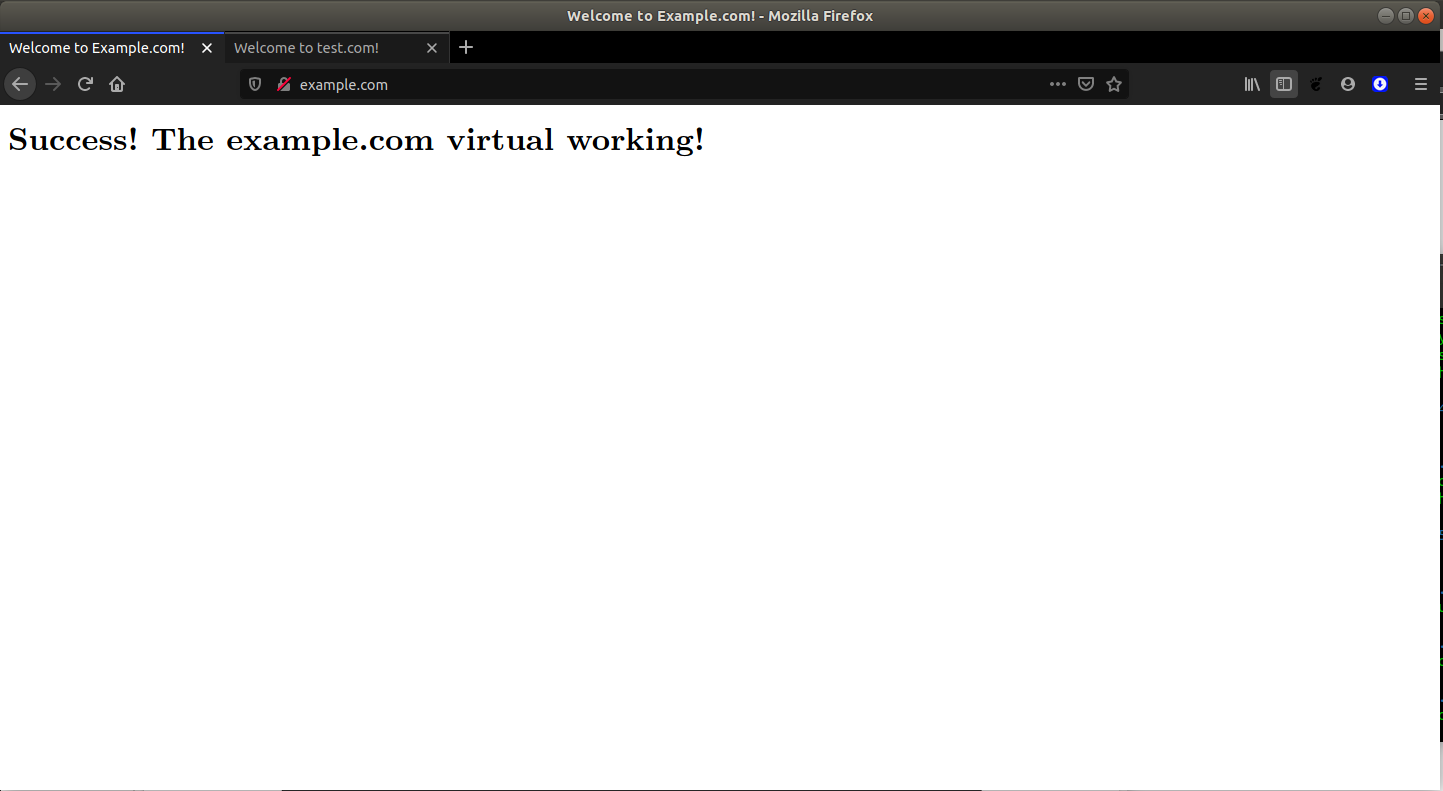
\includegraphics[width=\linewidth]{example-res.png}
    		\caption{When typing example.com}
  		\end{subfigure}
  		\begin{subfigure}[b]{0.4\linewidth}
    		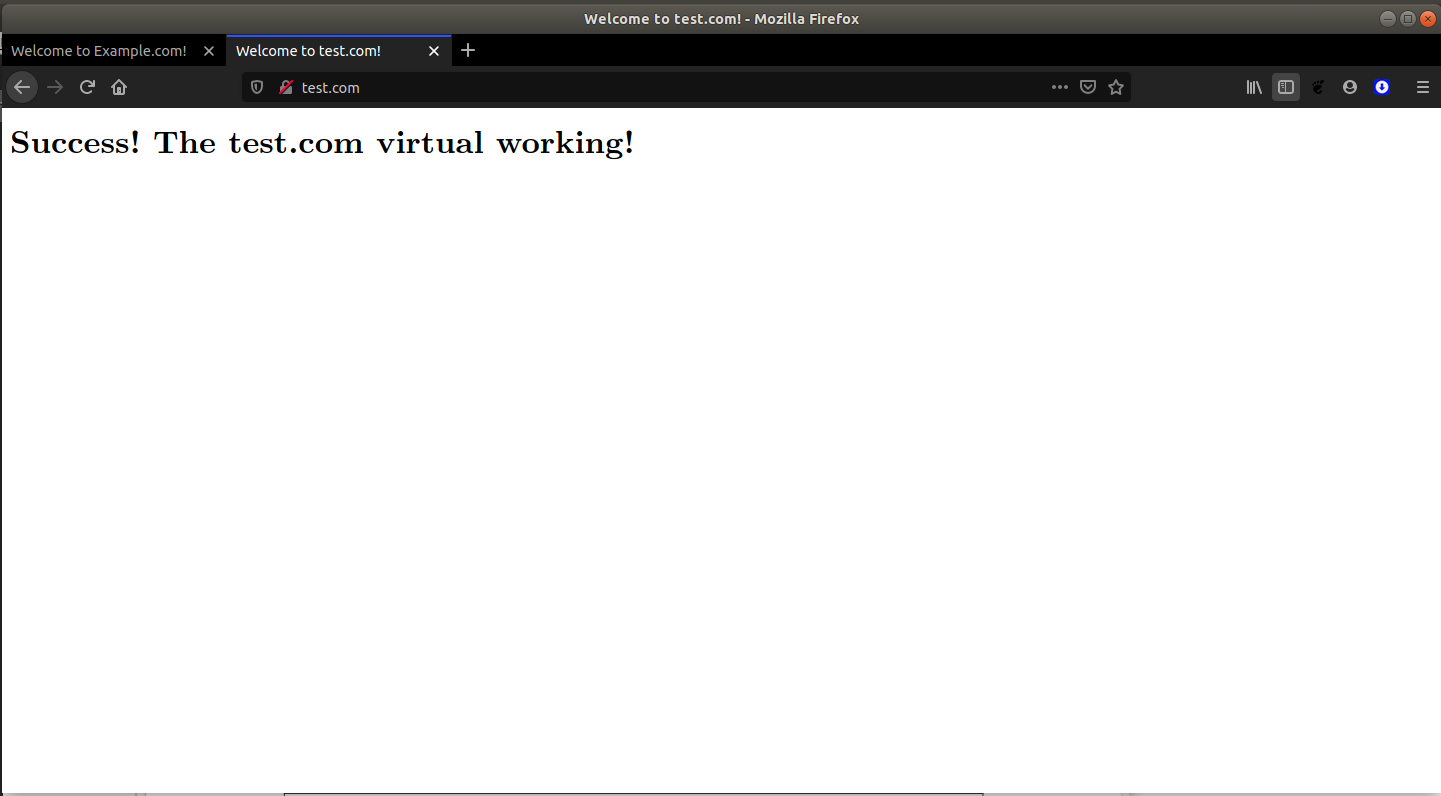
\includegraphics[width=\linewidth]{test-res.png}
    		\caption{When typing test.com}
  		\end{subfigure}
  		\caption{Result from web browser}
  		\label{fig:webbrowserres}
	\end{figure}
	\\Explain:\\
	When you ran two a2ensite commands for the two conf files, it will enable those two sites, which contained the information stored on the two html files above. After you reload apache to registered those changes and add the ip address (127.0.0.1 or localhost) and map it to the two websites.
	\\The results are showed above: when you type those 2 addresses to browser, it will show the html file.
	\section{Make others machine on LAN to connect to these two websites}
	\newpage
	\begin{enumerate}
		\item Type: "hostname -I" onto your terminal, you will see your local IP address (starting with 192.168.) and maybe a broadcast IP address of some other processes (like docker, if you installed) (starting with 172.). We only need the local IP address. We get the result like this:
		\begin{figure}[h!]
  			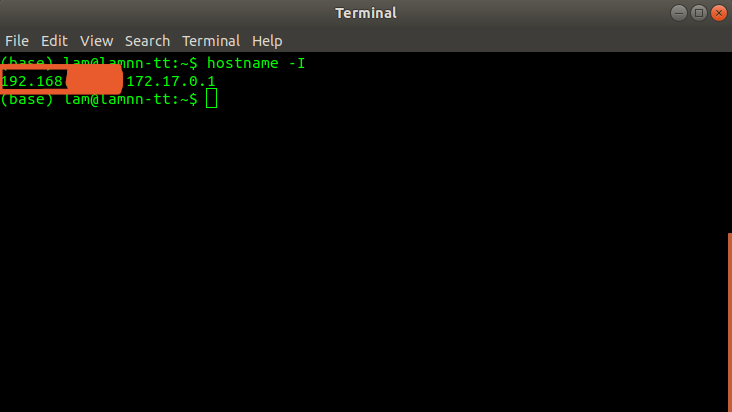
\includegraphics[width=\linewidth]{local-ip.png}
  			\caption{My local ip address}
  			\label{fig:loc-ip}
		\end{figure}
		\item On another computer on the same LAN, open the file /etc/hosts and add these lines with 192.168.x.x is the address you just obtained:\\
		"192.168.x.x example.com"\\
		"192.168.x.x test.com"
	\end{enumerate}
	\section{Code for the while loop}
	\begin{figure}[h!]
  		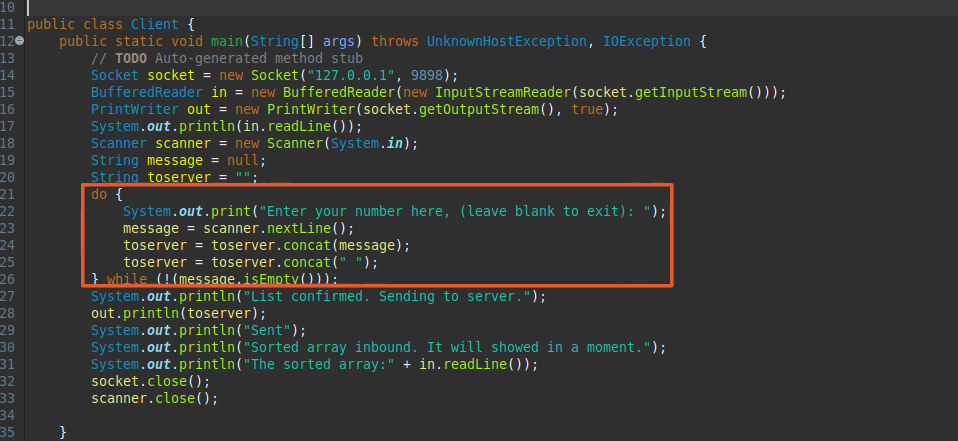
\includegraphics[width=\linewidth]{client-code.png}
  		\caption{My client-side}
  		\label{fig:client}
	\end{figure}
	\newpage
	\section{Role of method run()}
	\begin{itemize}
		\item Take the preprocessed input string from client-side.
		\item Split it in a string array.
		\item Parse each item in that array into integer, thus make an array of integer.
		\item Do the sort process (call class)
		\item Convert the integer array to String
		\item Send the result to Client and close socket.
	\end{itemize}
	\begin{figure}[h!]
  		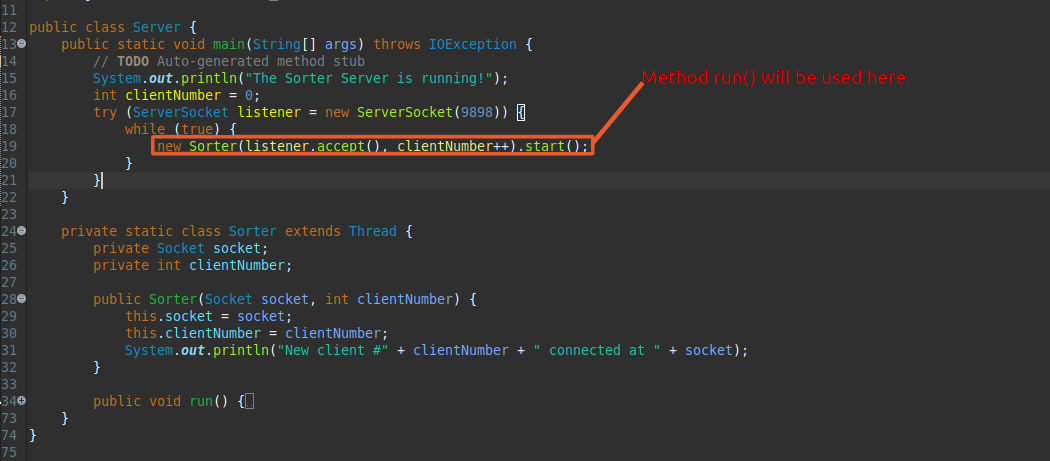
\includegraphics[width=\linewidth]{server-code.png}
  		\caption{My server side}
  		\label{fig:server}
	\end{figure}
	\section{Note}
	\begin{itemize}
		\item You can find my poject at: \href{https://github.com/lam1910/DistributedSystem}{Distributed System repository}
	\end{itemize}
	
	\chapter{Chapter 2 Lab Work: Architectures}
	\newpage
		\section{Commands Used}
  	\label{sec:cmd}
  	\begin{itemize}
  		\item snap install kubectl --classic
  		\item kubectl version
  		\item git clone https://github.com/anhth318/microservices-demo.git
  		\item cd path/to/the/cloned/repository/microservice-demo
  		\item ./mvnw clean package -Dmaven.test.skip=true
  		\item docker login
  		\item docker build --tag=microservice-kubernetes-demo-apache apache
  		\item docker tag microservice-kubernetes-demo-apache \emph{lam1910}/microservice-kubernetes-demo-apache:latest
  		\item docker push \emph{lam1910}/microservice-kubernetes-demo-apache
  		\item docker build --tag=microservice-kubernetes-demo-catalog microservice-kubernetes-demo-catalog
  		\item docker tag microservice-kubernetes-demo-catalog \emph{lam1910}/microservice-kubernetes-demo-catalog
		\item docker push \emph{lam1910}/microservice-kubernetes-demo-catalog
		\item docker build --tag=microservice-kubernetes-demo-customer microservice-kubernetes-demo-customer
		\item docker tag microservice-kubernetes-demo-customer \emph{lam1910}/microservice-kubernetes-demo-customer
		\item docker push \emph{lam1910}/microservice-kubernetes-demo-customer
		\item docker build --tag=microservice-kubernetes-demo-order microservice-kubernetes-demo-order
		\item docker tag microservice-kubernetes-demo-order \emph{lam1910}/microservice-kubernetes-demo-order:lastest
		\item docker push \emph{lam1910}/microservice-kubernetes-demo-order
  	\end{itemize}
  	\section{Changes in Dockerhub Website}
  	\label{sec:change}
  	As you can see from \ref{fig:dockerhubrepo}, after you run all the the commands from \ref{sec:cmd}, you will have 4 repositories in your account's repositories\footnote{You can find out more at \href{https://hub.docker.com/u/lam1910}{My Docker}}.
  	\begin{figure}[p]
		\centering
  		\begin{subfigure}[b]{\linewidth}
    		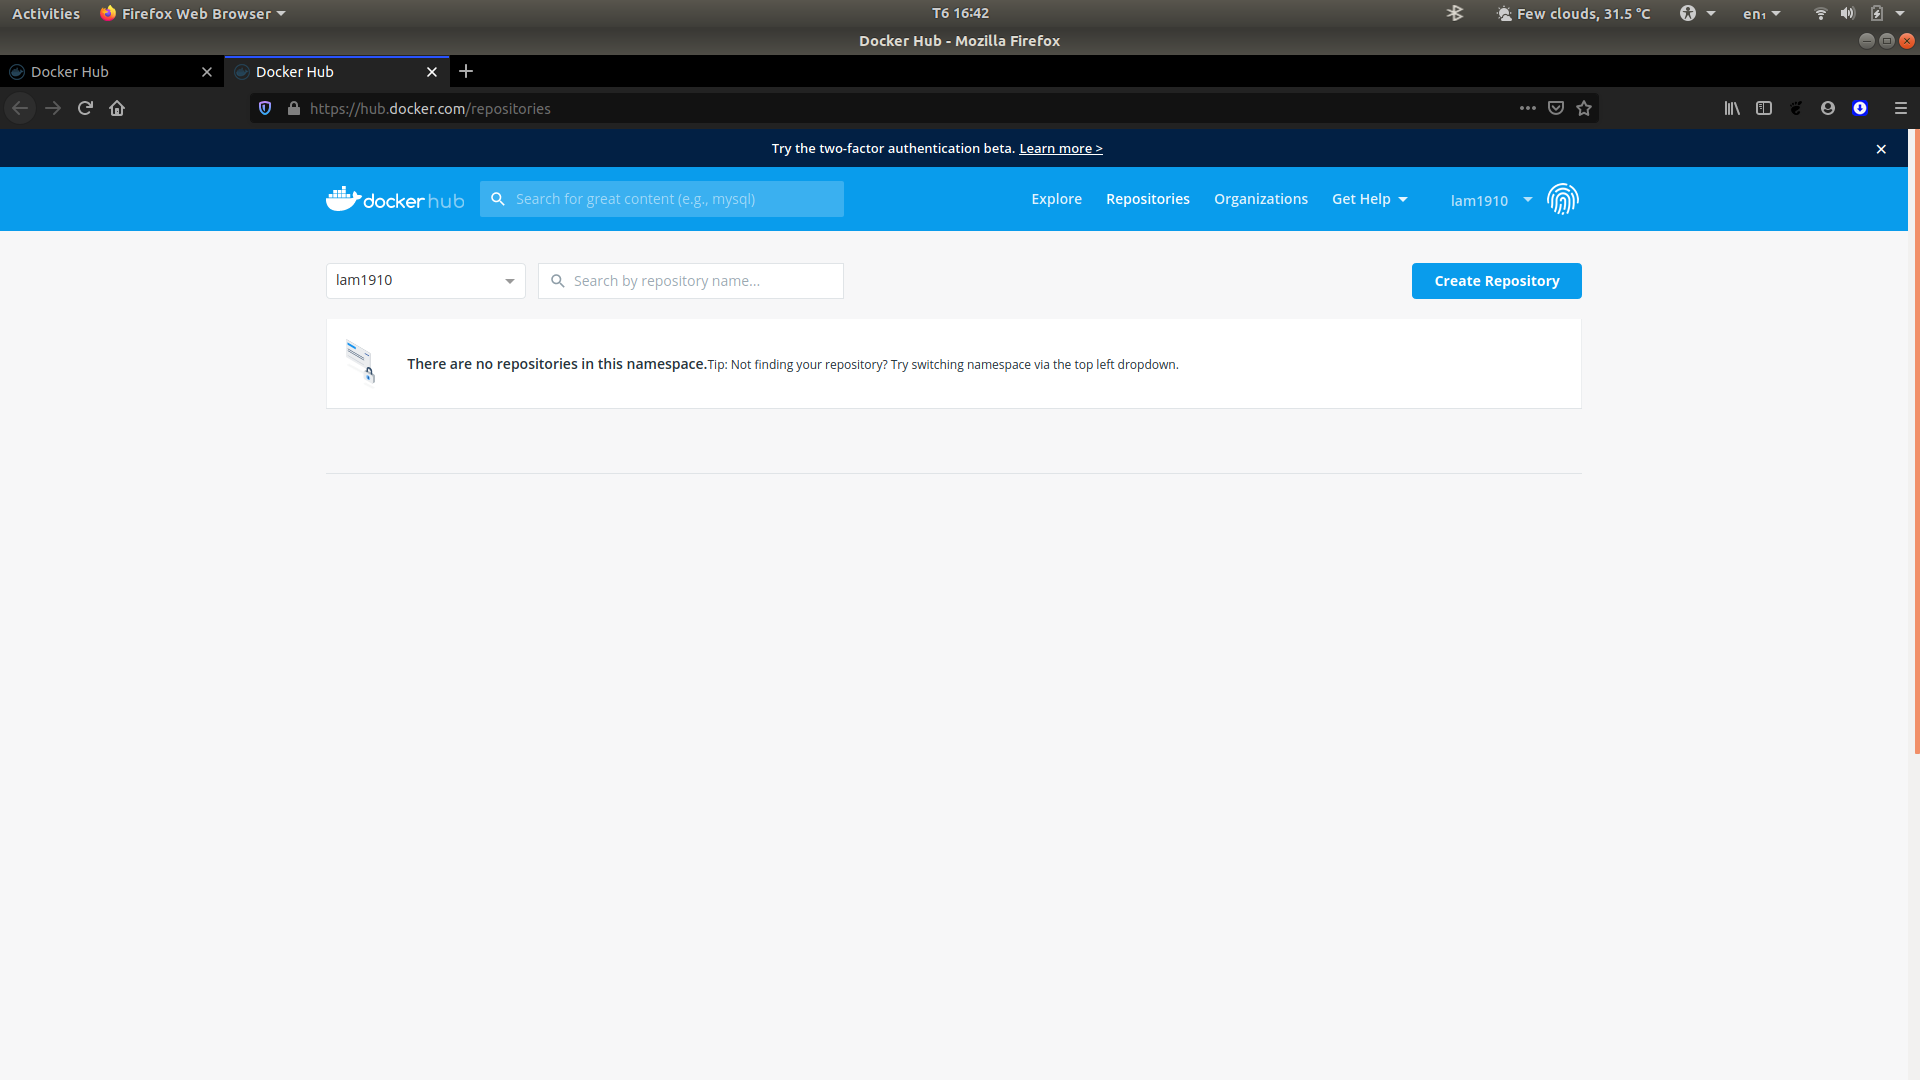
\includegraphics[width=\linewidth]{docker-repo-before.png}
    		\caption{Before pushing anything}
  		\end{subfigure}
  		\begin{subfigure}[b]{\linewidth}
    		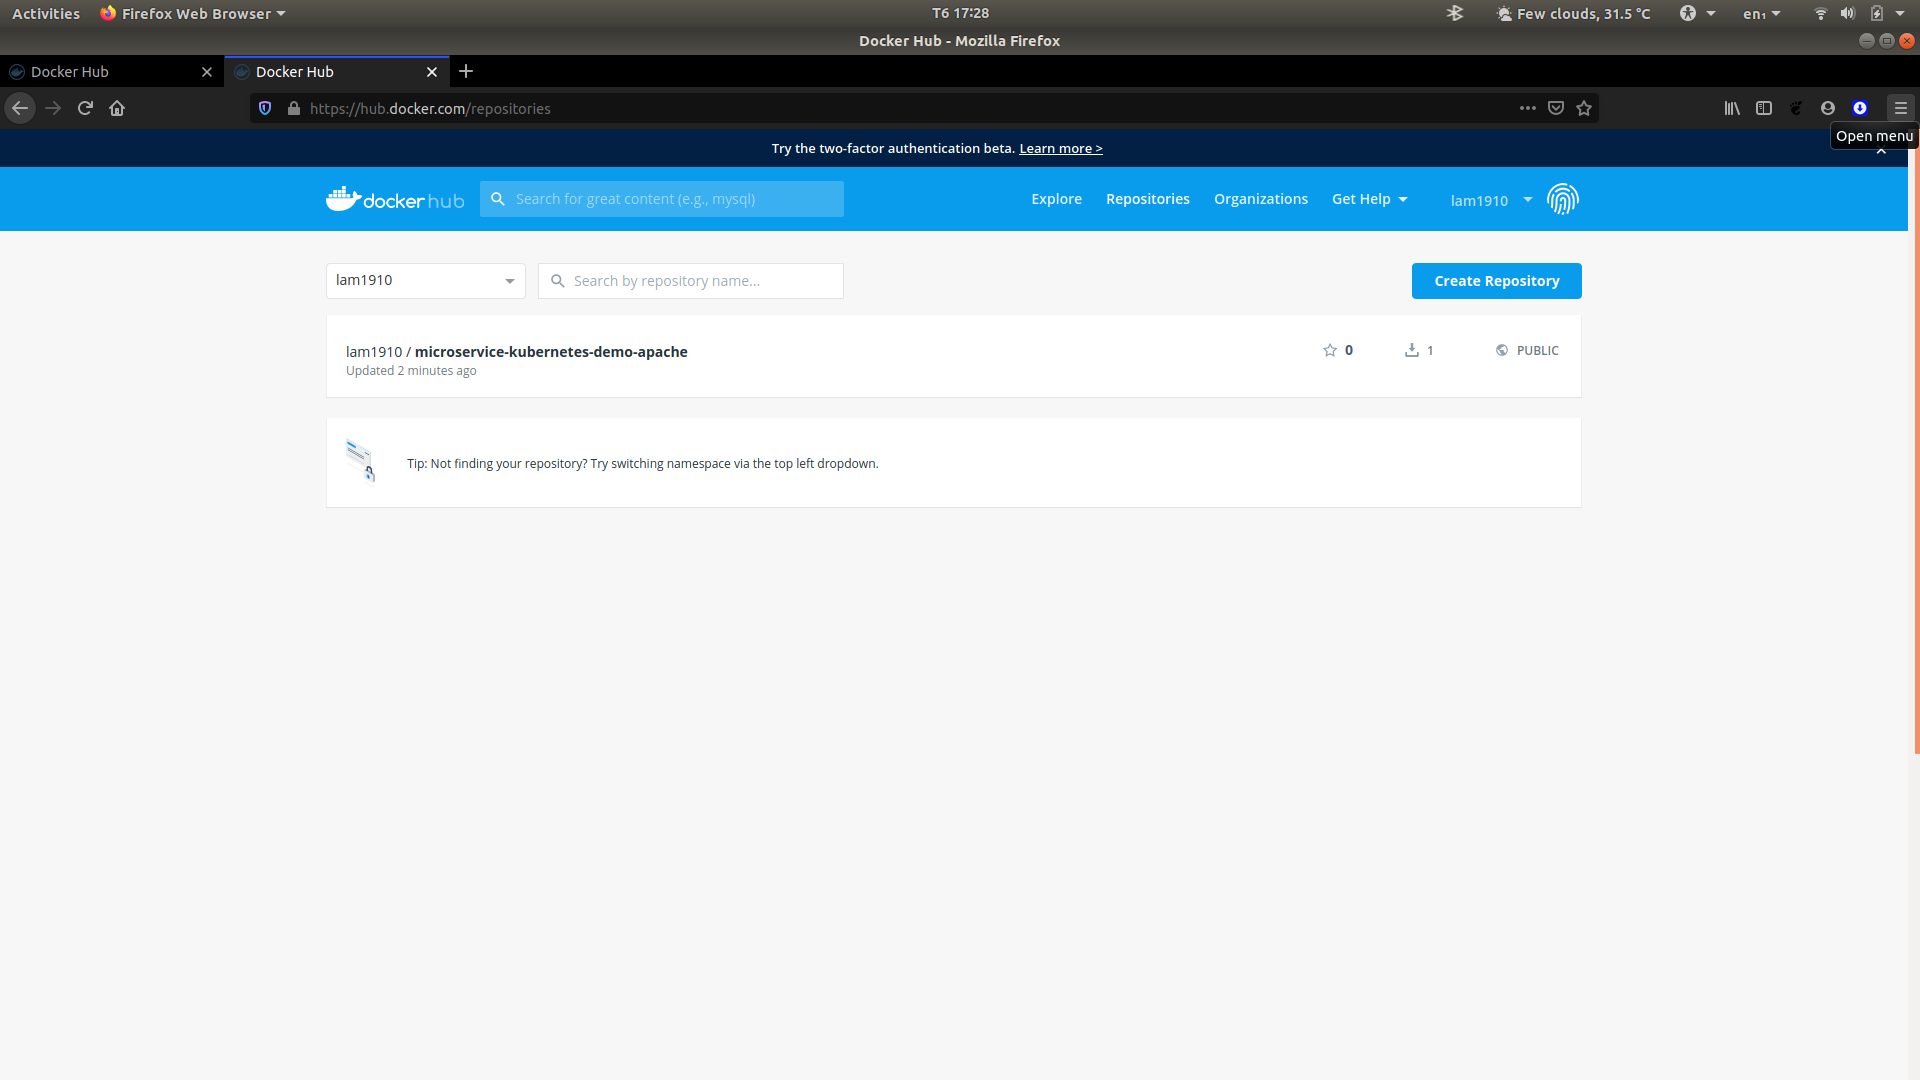
\includegraphics[width=\linewidth]{docker-repo-after.png}
    		\caption{After pushing one service}
  		\end{subfigure}
  		\begin{subfigure}[b]{\linewidth}
    		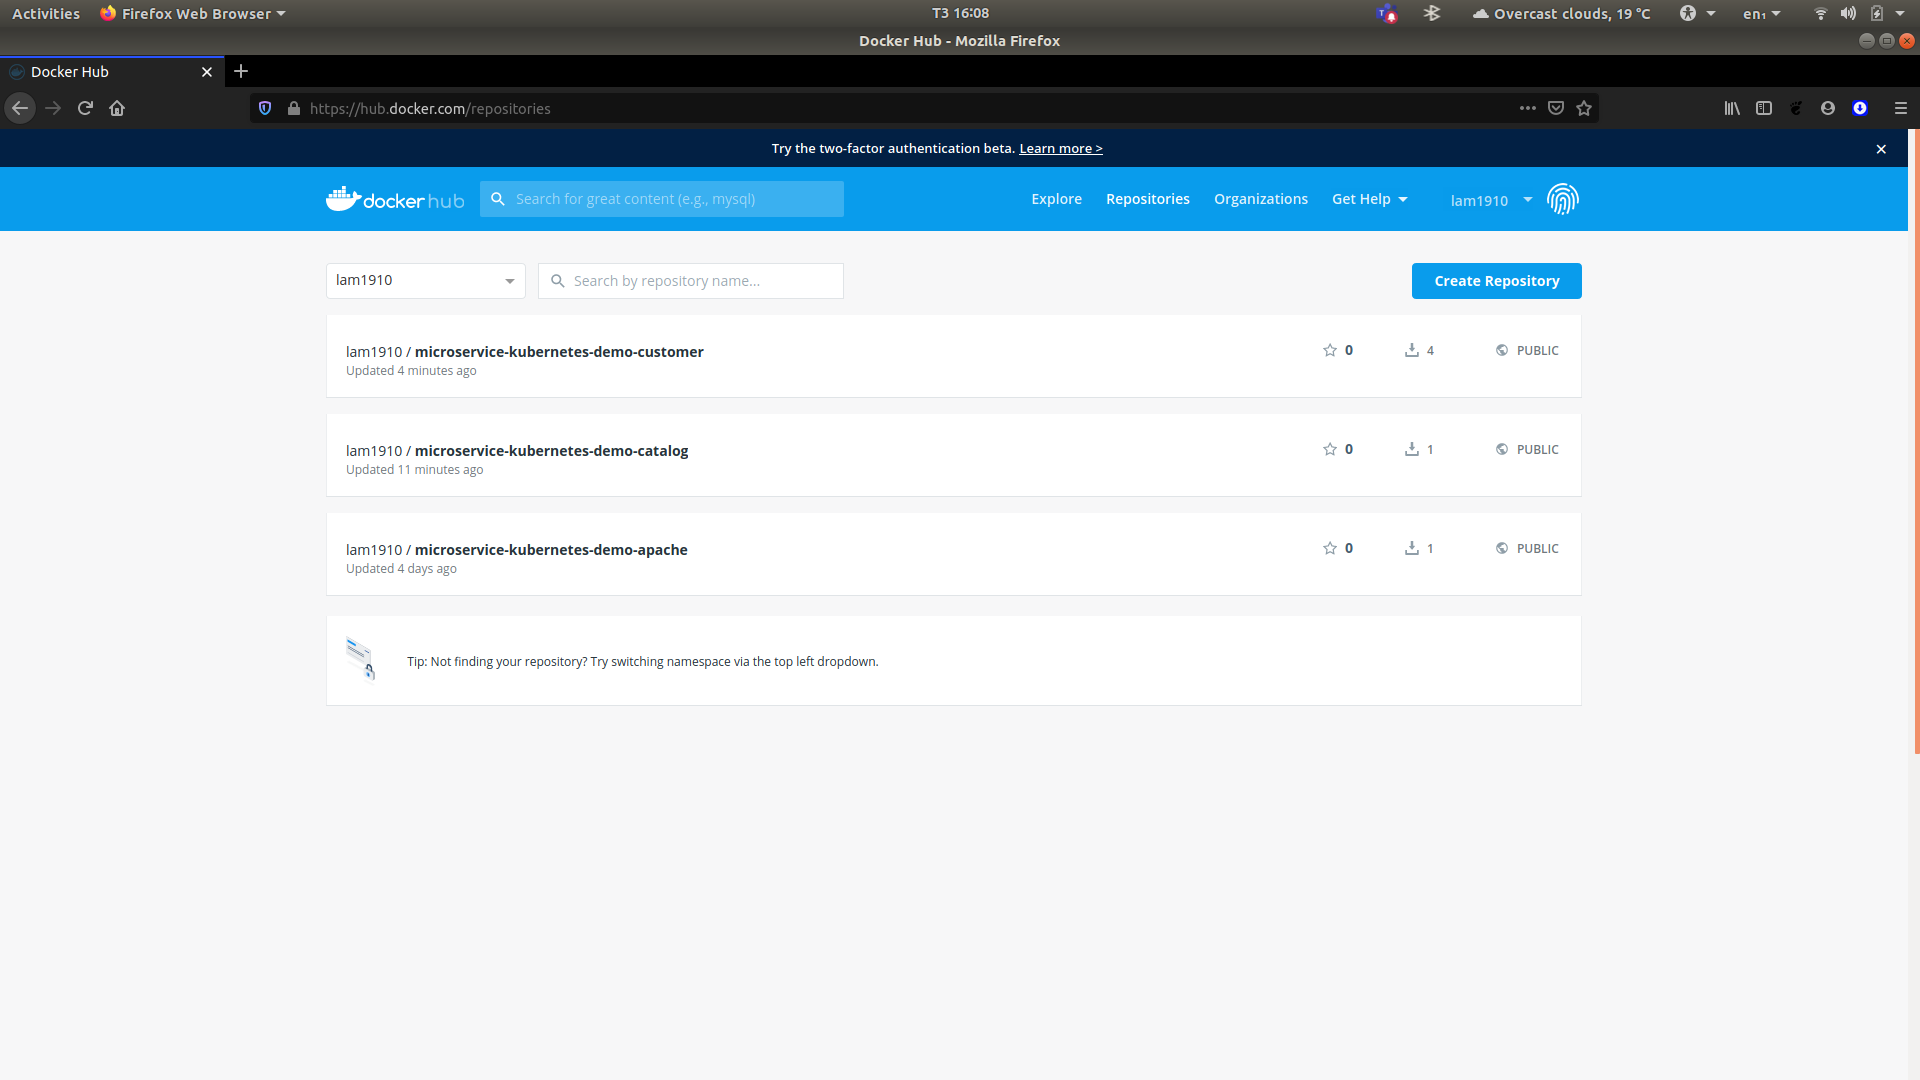
\includegraphics[width=\linewidth]{docker-end-push.png}
    		\caption{After pushing all services}
  		\end{subfigure}
  		\caption{Result from web browser}
  		\label{fig:dockerhubrepo}
	\end{figure}

	\newpage
	\section{Status of Pods}
	\label{sec:stpod}
  	\begin{figure}[h!]
		\centering
  		\begin{subfigure}[b]{0.4\linewidth}
  		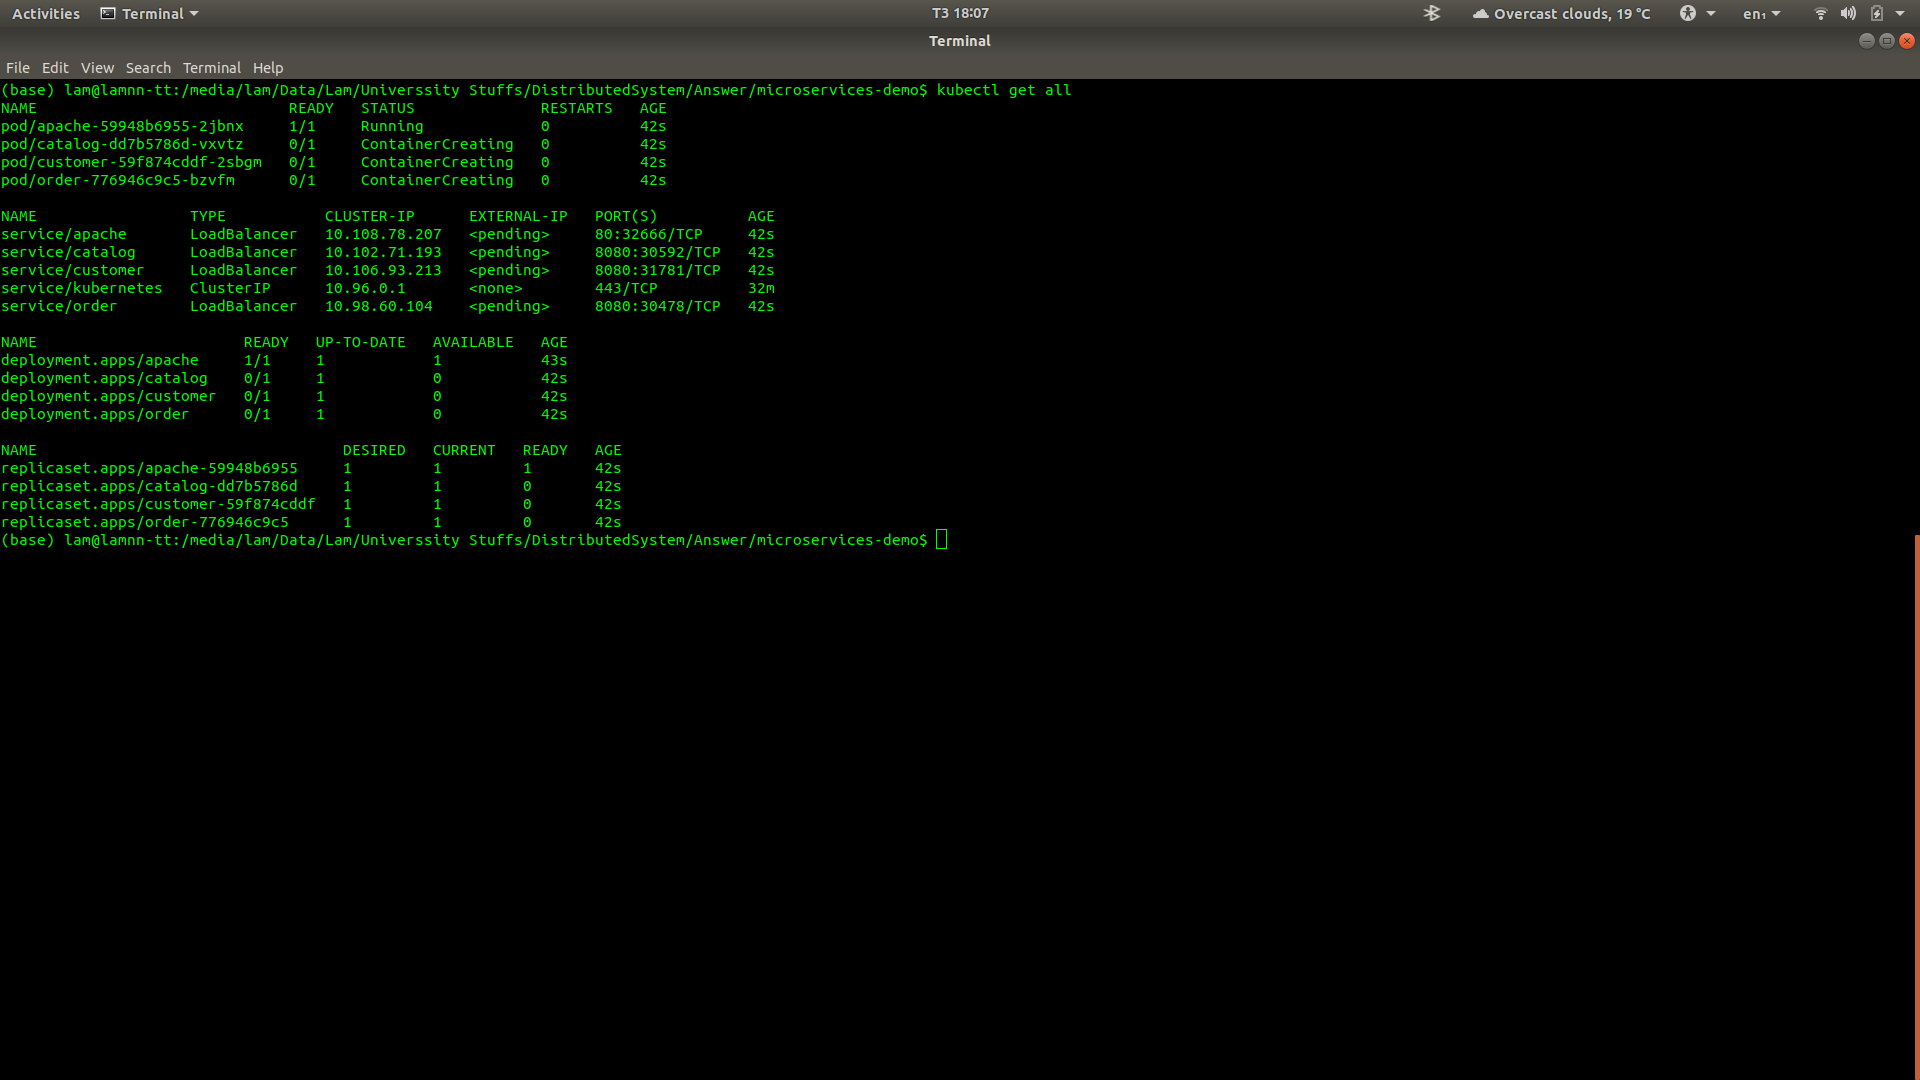
\includegraphics[width=\linewidth]{status-at34.png}
    		\caption{Pods status at second 34th}
  		\end{subfigure}
  		\begin{subfigure}[b]{0.4\linewidth}
    		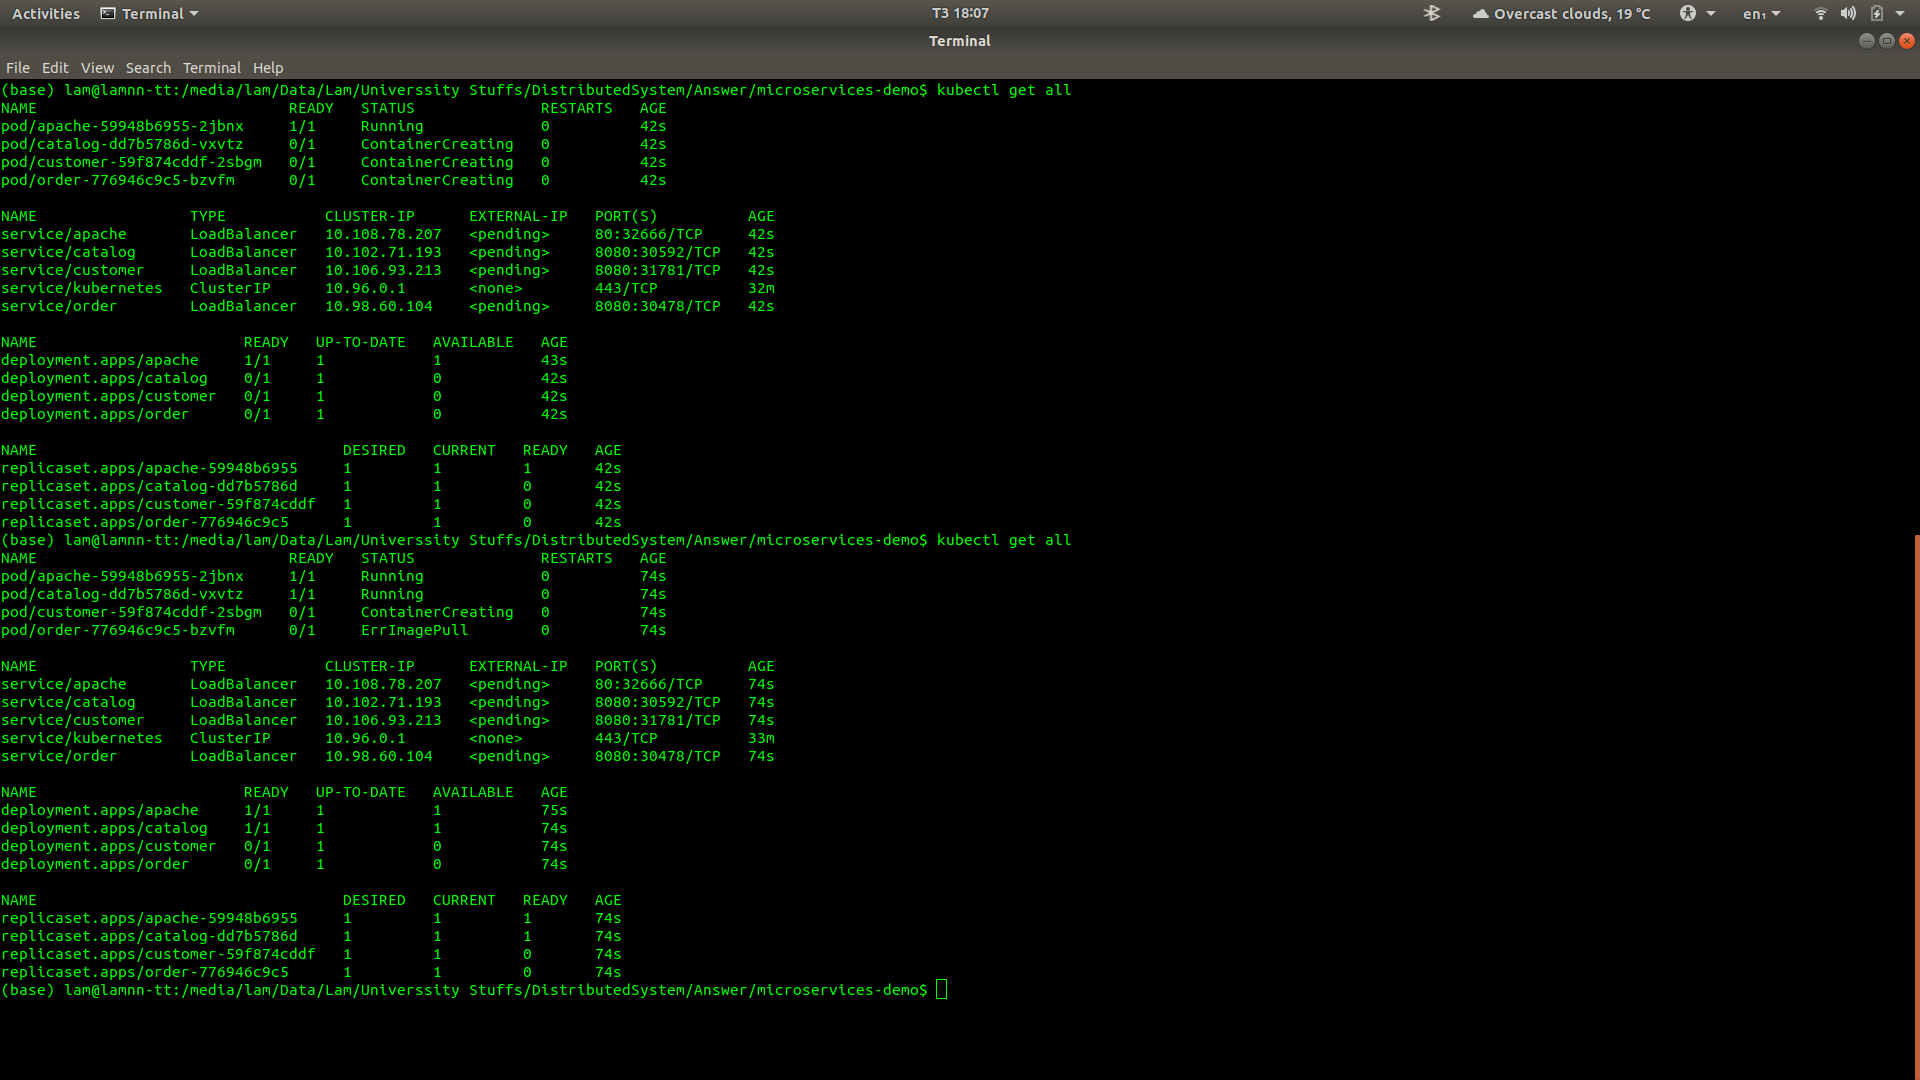
\includegraphics[width=\linewidth]{status-at74.png}
    		\caption{Pods status at second 74th}
  		\end{subfigure}
  		\caption{Status of pods at two time slots}
  		\label{fig:podstat}
	\end{figure}
	The different between two timeframe from \ref{fig:podstat} is that the age of the pods.
	\section{Role of Application Server Glassfish}
	\label{sec:glassfish}
	Glassfish Server is a webserver to deploy web application that was written in java. It uses the Message Queue software as its native JMS provide, providing transparent JMS messaging support.
	\section{Role of the Two JNDIs}
	\label{sec:jndi}
	By making calls to the JNDI API, applications locate resources and other program objects. Each resource object is identified by a unique, people-friendly name, called the JNDI name. A resource object and its JNDI name are bound together by the naming and directory service, which is included with the GlassFish Server. JNDI allows distributed applications to look up services in an abstract, resource-independent way.
	\begin{figure}[h!]
		\centering
  		\begin{subfigure}[b]{0.4\linewidth}
  		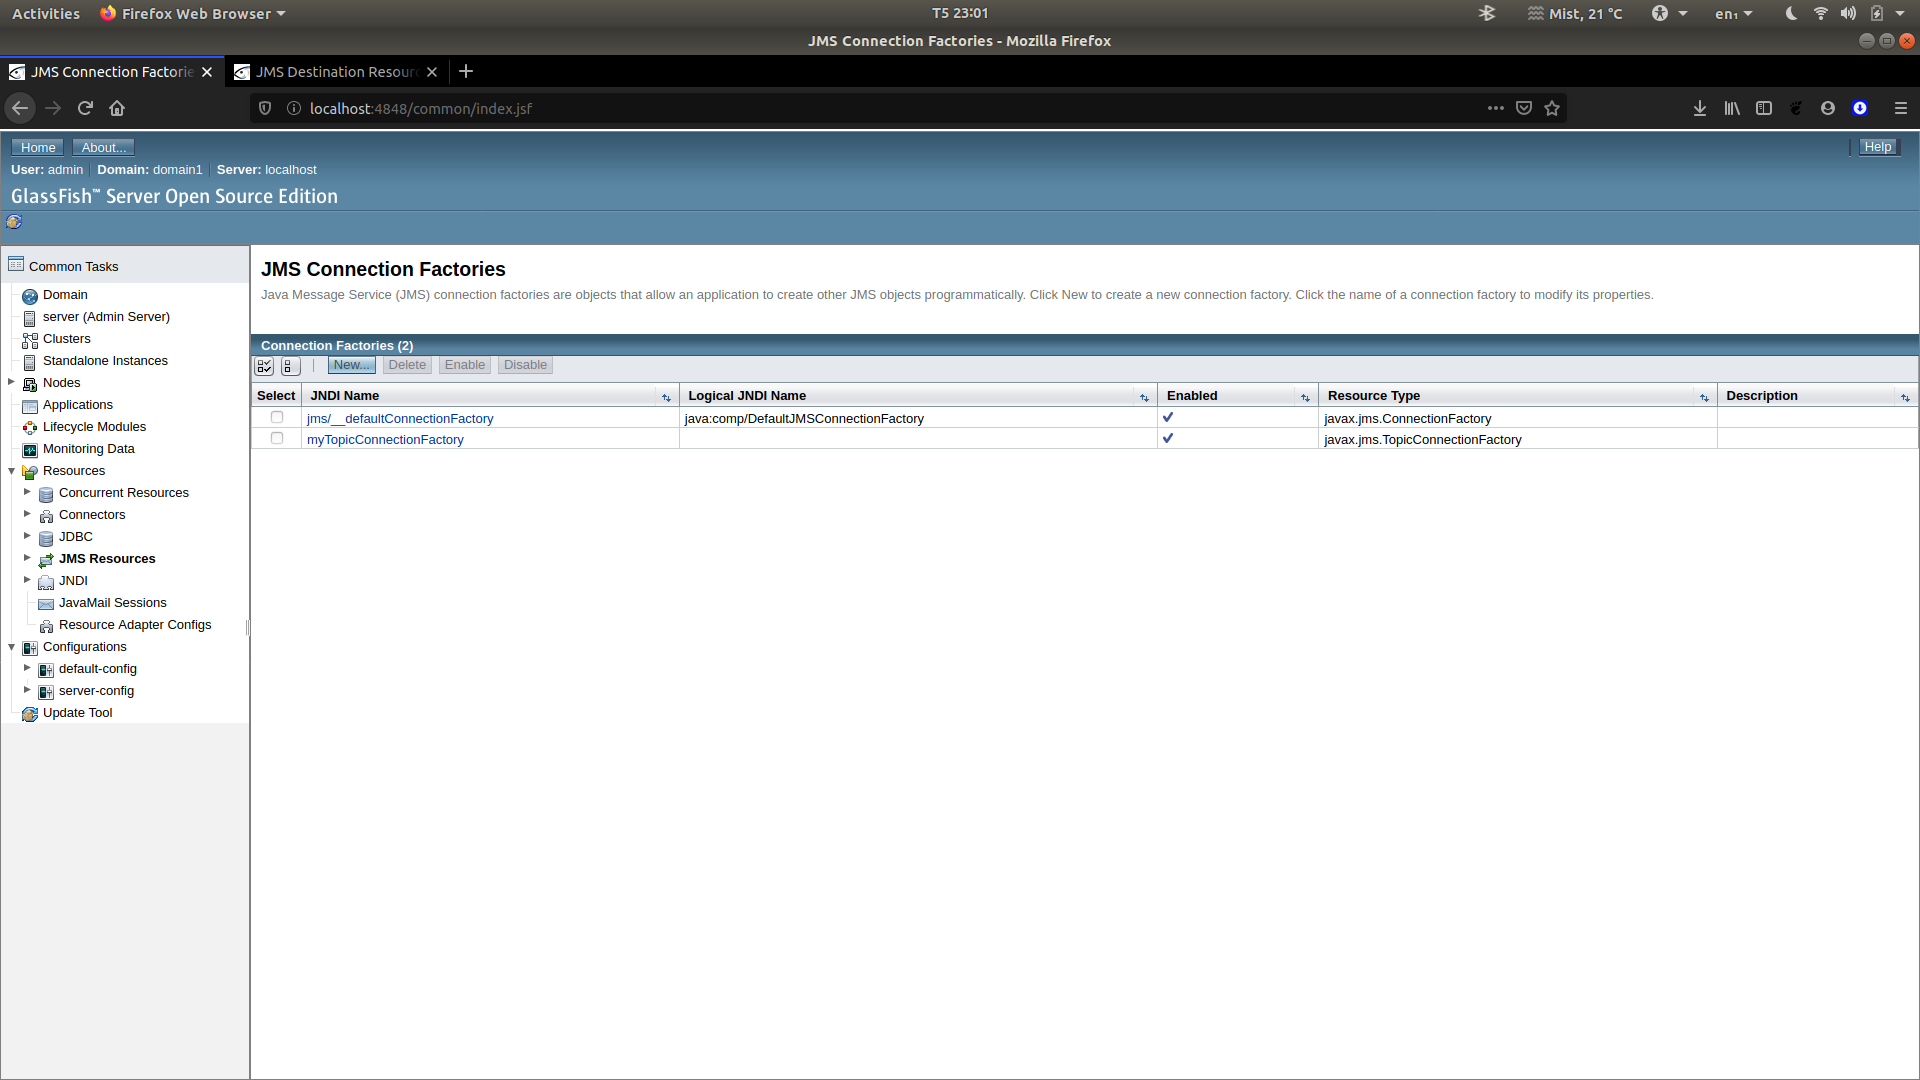
\includegraphics[width=\linewidth]{jndi1.png}
    		\caption{JMS Connection Factories}
  		\end{subfigure}
  		\begin{subfigure}[b]{0.4\linewidth}
    		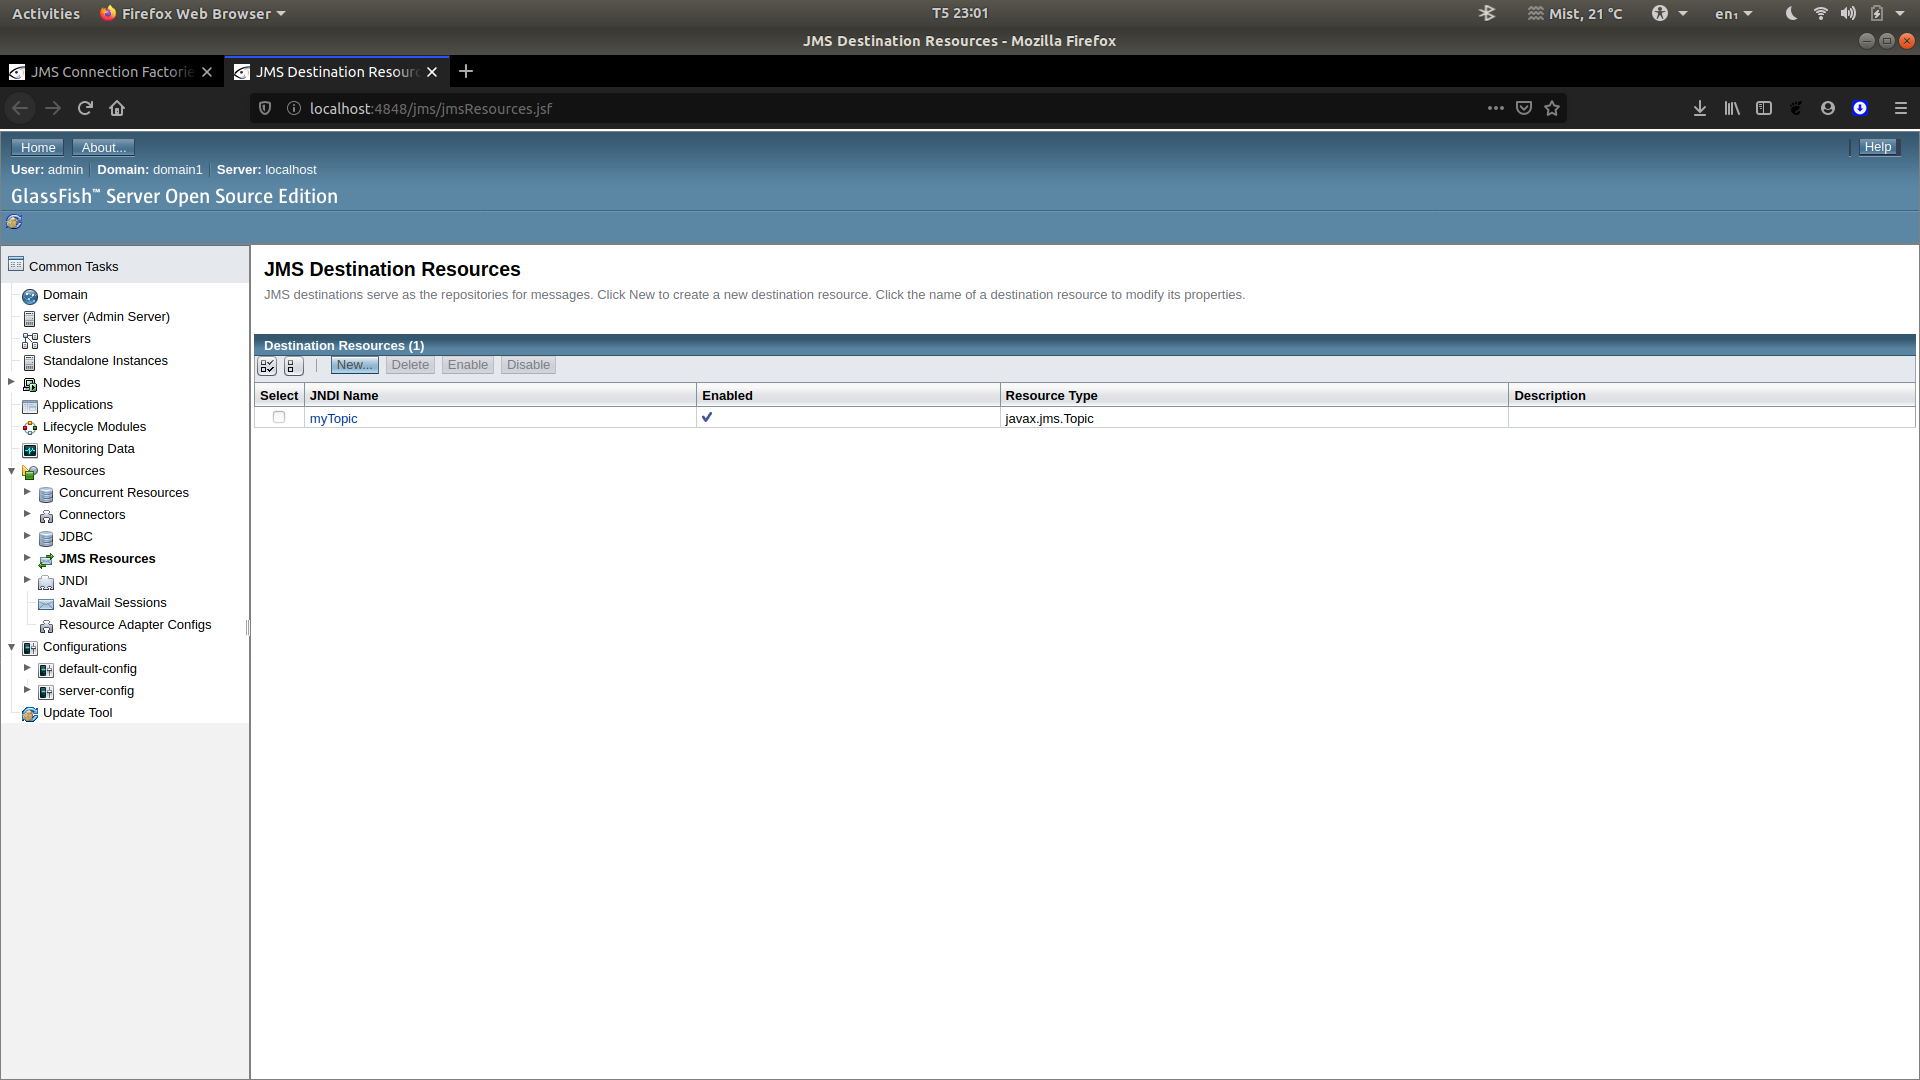
\includegraphics[width=\linewidth]{jndi2.png}
    		\caption{JMS Destination Resources}
  		\end{subfigure}
  		\caption{JNDIs}
  		\label{fig:jndi}
	\end{figure}
	\section{The Message Passing Method of Sender and Receiver Explaination}
	\label{sec:mespassexpl}
	\begin{figure}[h!]
		\centering
  		\begin{subfigure}[b]{0.4\linewidth}
  		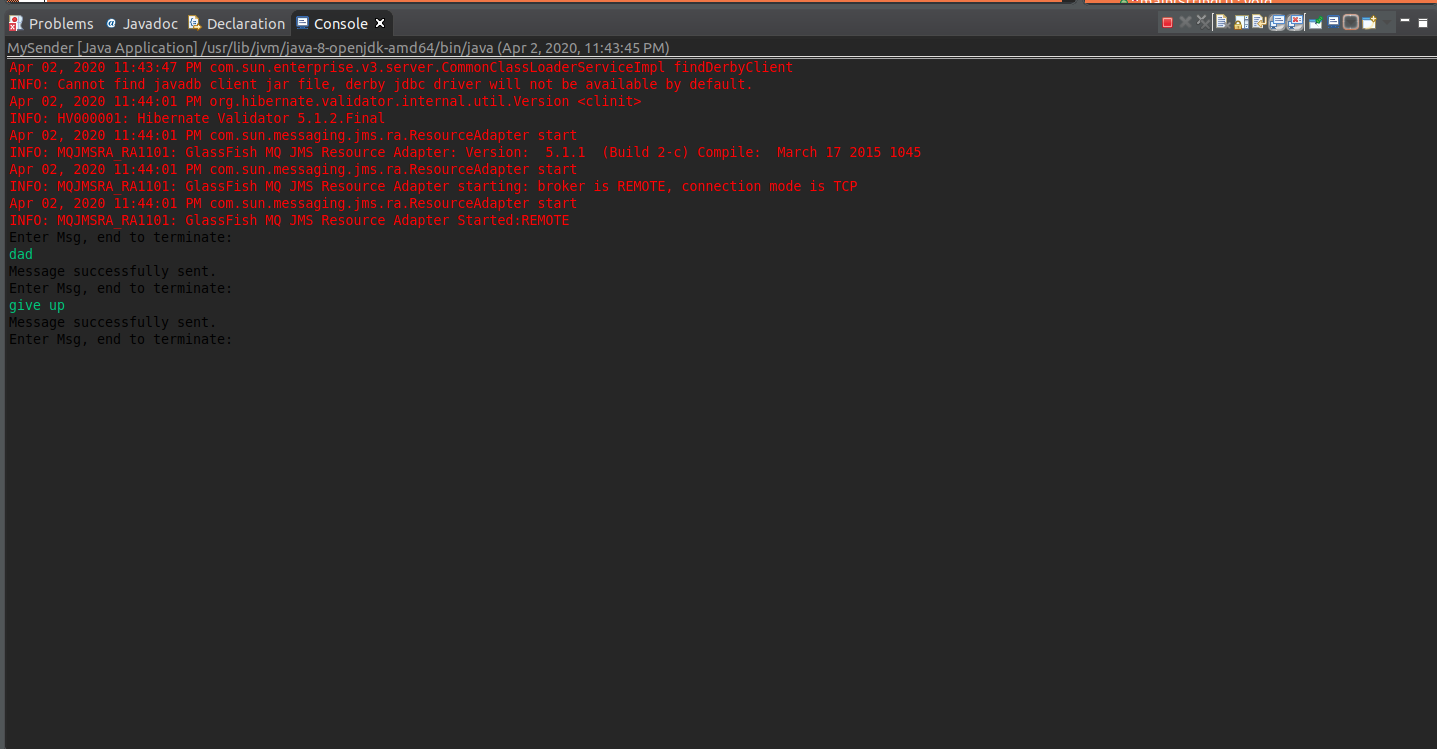
\includegraphics[width=\linewidth]{sender-res.png}
    		\caption{Sender}
  		\end{subfigure}
  		\begin{subfigure}[b]{0.4\linewidth}
    		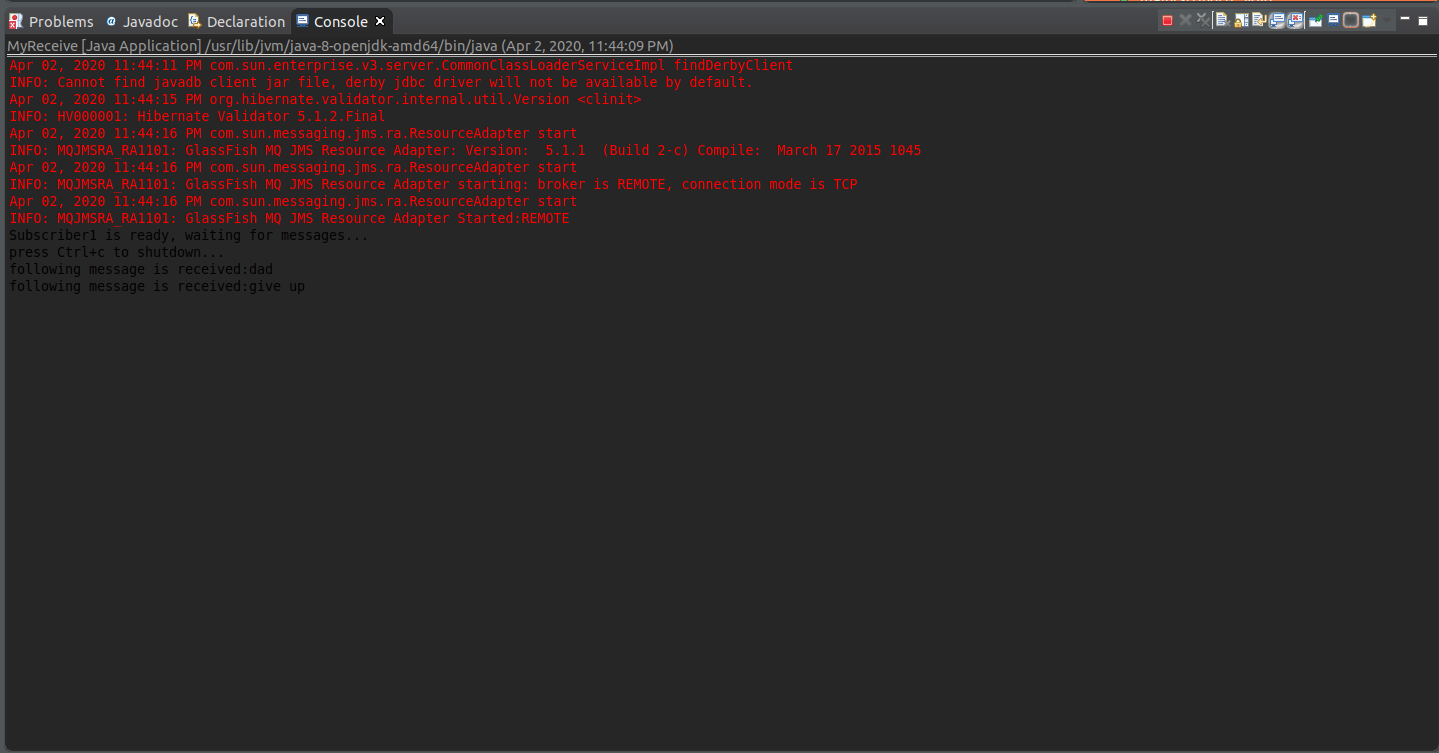
\includegraphics[width=\linewidth]{receiver-res.png}
    		\caption{Receiver}
  		\end{subfigure}
  		\caption{Result of running MySender and MyReceiver}
  		\label{fig:jndi}
	\end{figure}
	Explanation:
	\begin{enumerate}
		\item The Sender get the topic object named ''myTopic''
		\item It creates a publisher to register that event
		\item It creates buffer to store user input and publish the message to subscribers of event ''myTopic''
		\item In regard to the Receiver, it subscriber to ''myTopic'' and be able to receive the Sender’s message
		\item When the Sender publishes the message, since the Receiver has already subscribed to that event and get that message
	\end{enumerate}
	\section{Compare the JMS and DDS}
	\begin{tabular}{|c|c|}
	\hline 
	JMS & DDS \\ 
	\hline 
	Java Messaging Service & Data Distributed Service \\ 
	\hline 
	Used for sending messages & DDS is networking middleware \\ between two or more clients & that simplifies complex \\&network programming. \\&It implements a \\& publish/subscribe model  \\&for sending and receiving data, \\&events, and commands among nodes. \\
	\hline 
	Centralized & Decentralized \\ 
	\hline 
	Allows the communication between & Automatically handles all\\ different components of  & aspects of message delivery \\ a distribute application &\\
	\hline 
	\end{tabular}
	
	\chapter{Chapter 3 Lab Work: Processes and Threads}
	\newpage
	\section{New File on ChatRoomApp folder}
  	The new file in said folder is package.json. This file holds various metadata relevant to the project. This file is used to give information to npm that allows it to identify the project as well as handle the project's dependencies. It can also contain other metadata such as a project description, the version of the project in a particular distribution, license information, even configuration data - all of which can be vital to both npm and to the end users of the package. The package.json file is normally located at the root directory of a Node.js project.
  	\begin{figure}[h!]
		\centering
  		\begin{subfigure}[b]{0.4\linewidth}
  		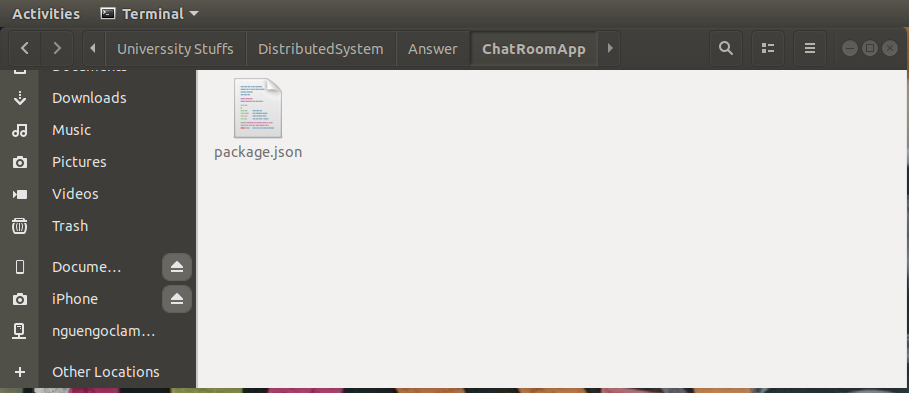
\includegraphics[width=\linewidth]{files-expl-chat.png}
    		\caption{File Explorer}
  		\end{subfigure}
  		\begin{subfigure}[b]{0.4\linewidth}
    		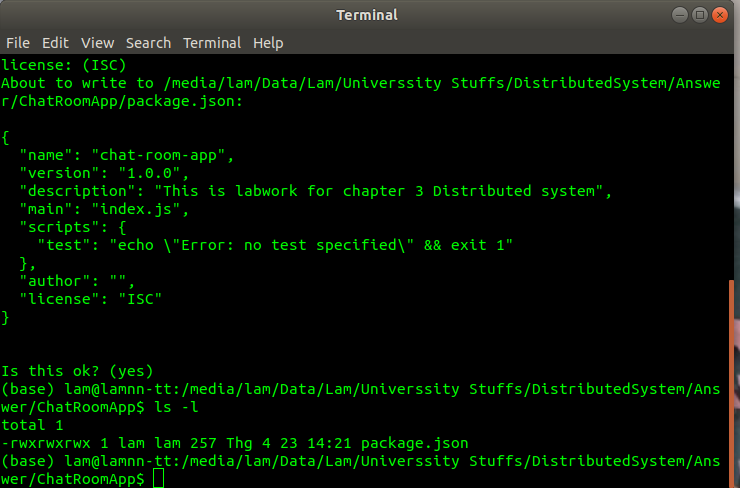
\includegraphics[width=\linewidth]{term-chat.png}
    		\caption{In terminal}
  		\end{subfigure}
  		\caption{New file}
  		\label{fig:pack}
	\end{figure}
	
	\section{Message On Port 3000}
	If you access to '127.0.0.1:3000' (or localhost:3000), the display message on the screen is hello world in plain text.
	\begin{figure}[h!]
  		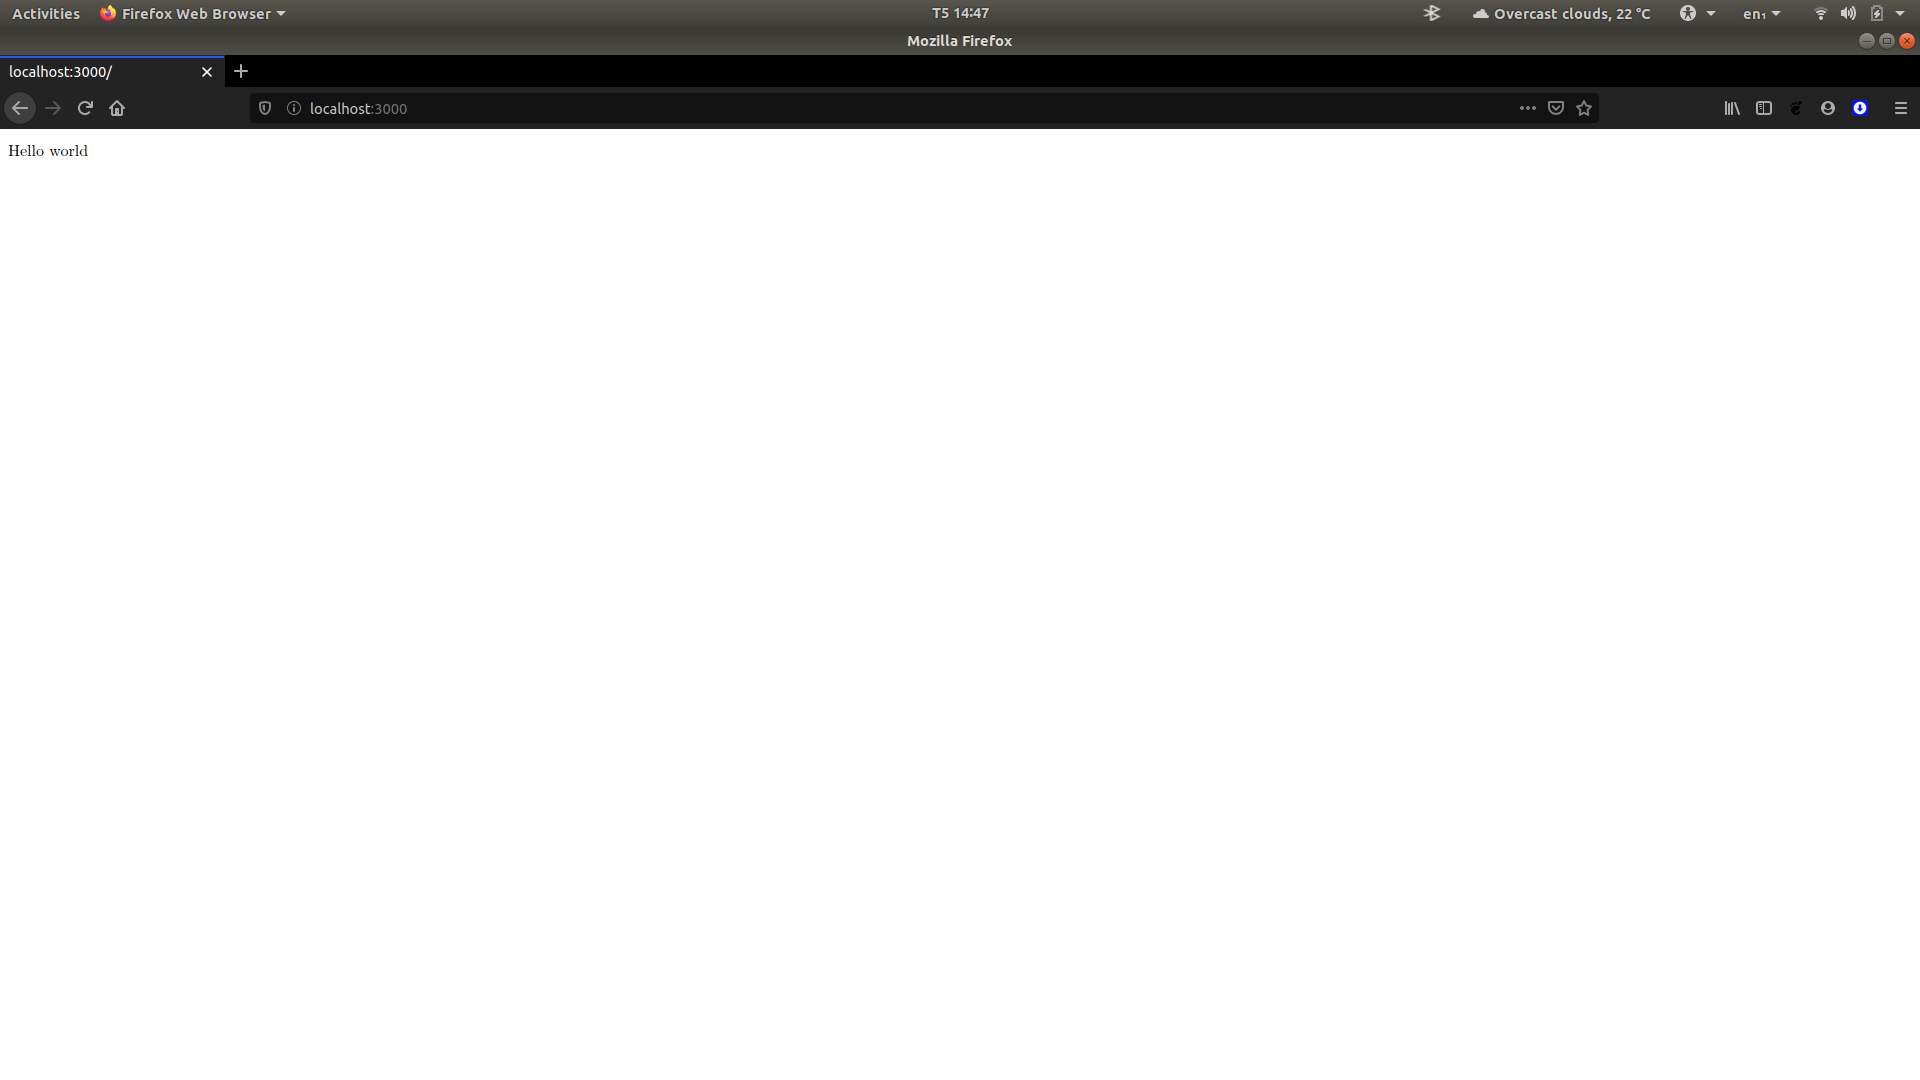
\includegraphics[width=\linewidth]{mess-on-port-3k.png}
  		\caption{Screenshot of the web browser}
  		\label{fig:hello}
	\end{figure}
	\newpage
	\section{Try Reload the Web Browser After Added socket.io}
	The console does not change since it is stil 1 'user' that conected to print hello world
	\begin{figure}[h!]
  		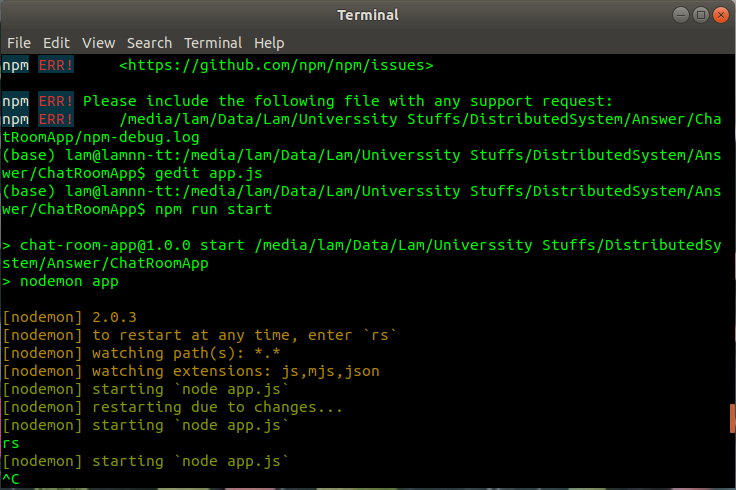
\includegraphics[width=\linewidth]{reload-web-before.png}
  		\caption{Screenshot of the console after added socket.io}
  		\label{fig:console1}
	\end{figure}
	
	\section{Try Reload the Web Browser After Fixed the Route and Added Style}
	This time, there is 'New User Connected' on the console
	\begin{figure}[h!]
  		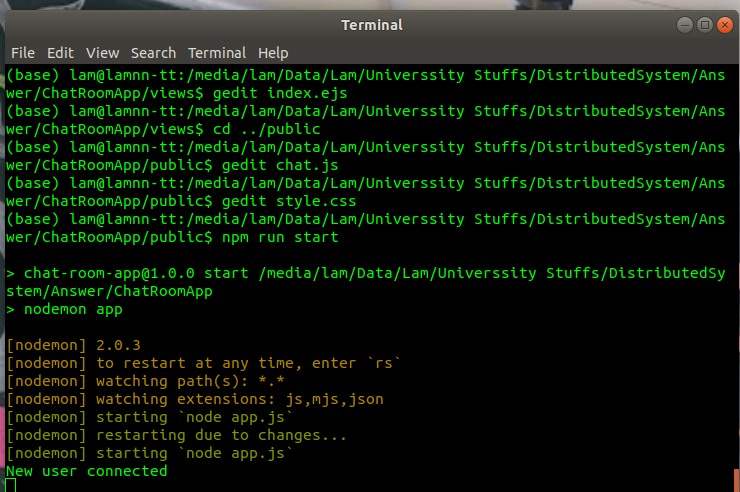
\includegraphics[width=\linewidth]{reload-web-after.png}
  		\caption{Screenshot of the console after fixed route and added style}
  		\label{fig:console2}
	\end{figure}
	
	\section{End Product}
	When 1 user is typing somthing on his or her instance, other people can see the line '$<$username$>$ is typing a message..' on top of the chatbox, in italic. When said user send the message, everyone will see a box with content as $<$username$>$: $<$message$>$ in blue.
	\begin{figure}[h!]
		\centering
  		\begin{subfigure}[b]{0.4\linewidth}
  		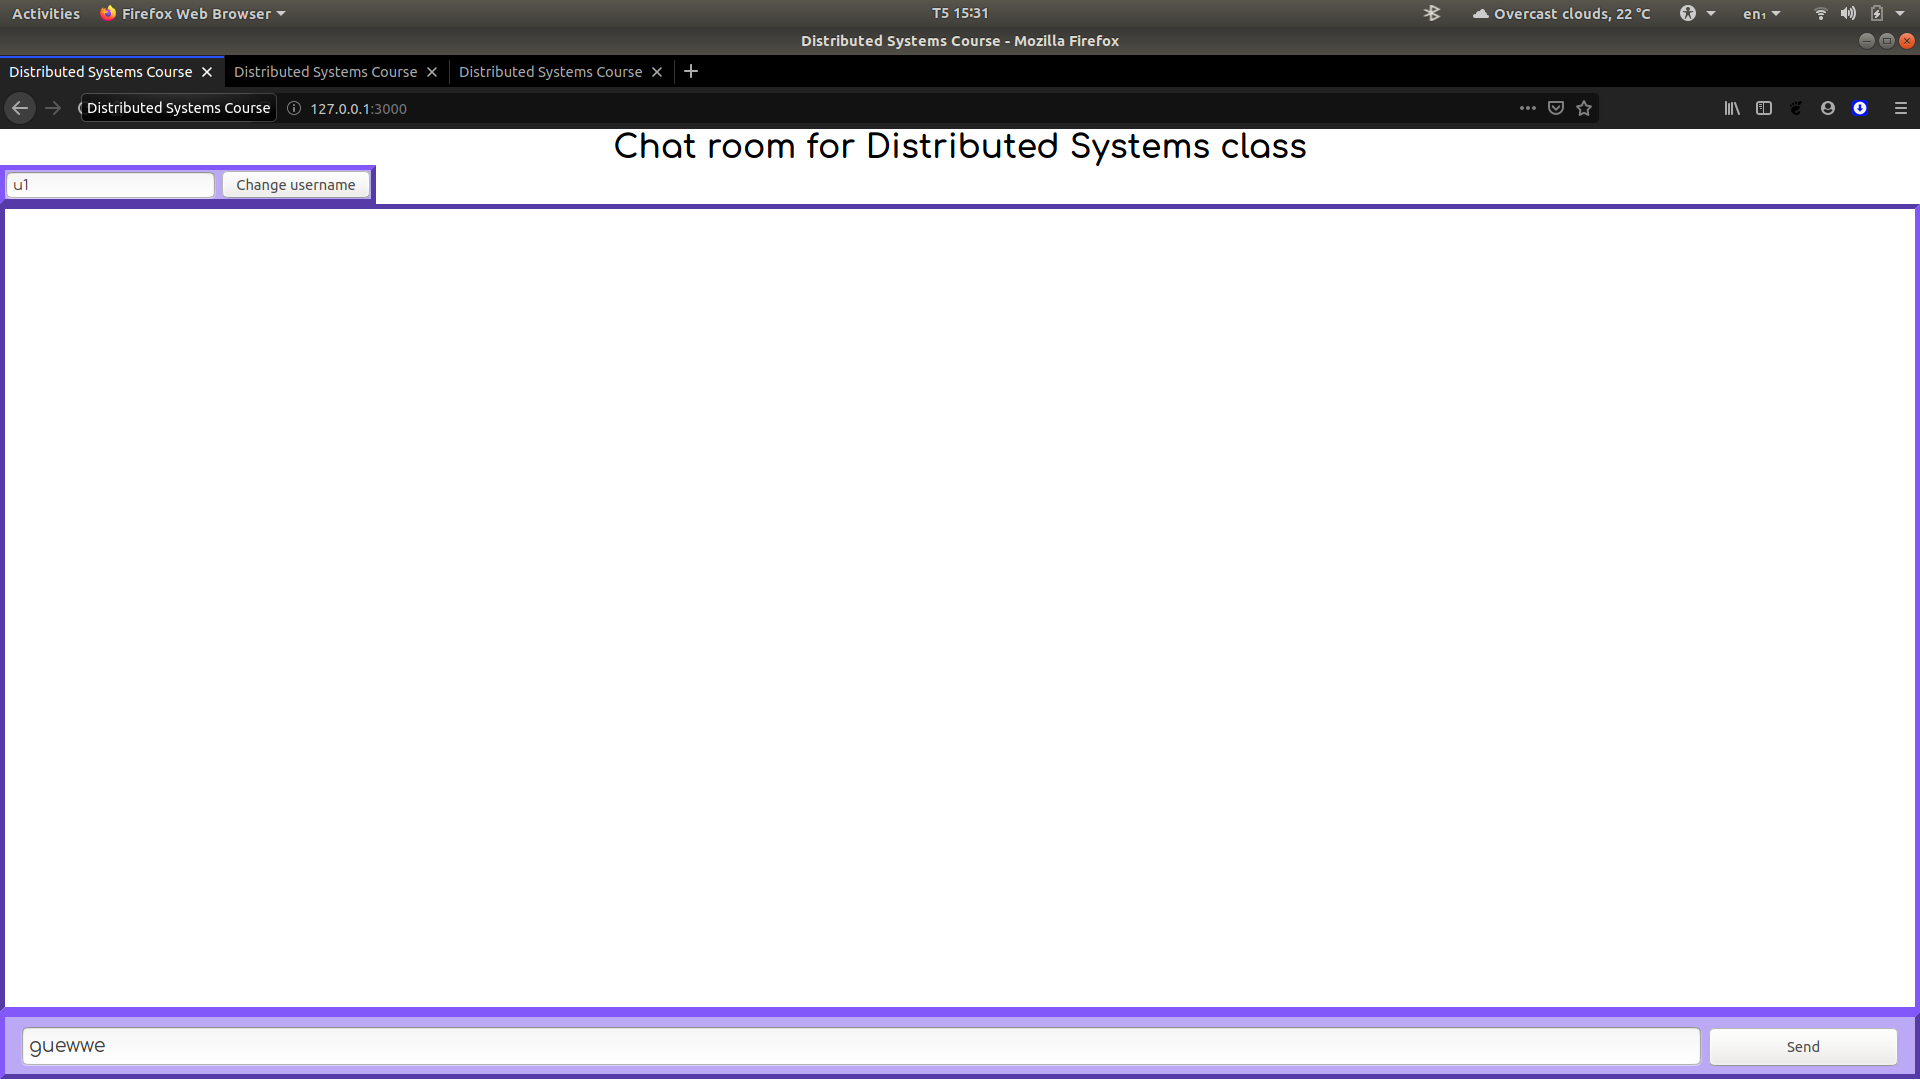
\includegraphics[width=\linewidth]{u1-type-notsend.png}
    		\caption{User u1 is typing}
  		\end{subfigure}
  		\begin{subfigure}[b]{0.4\linewidth}
    		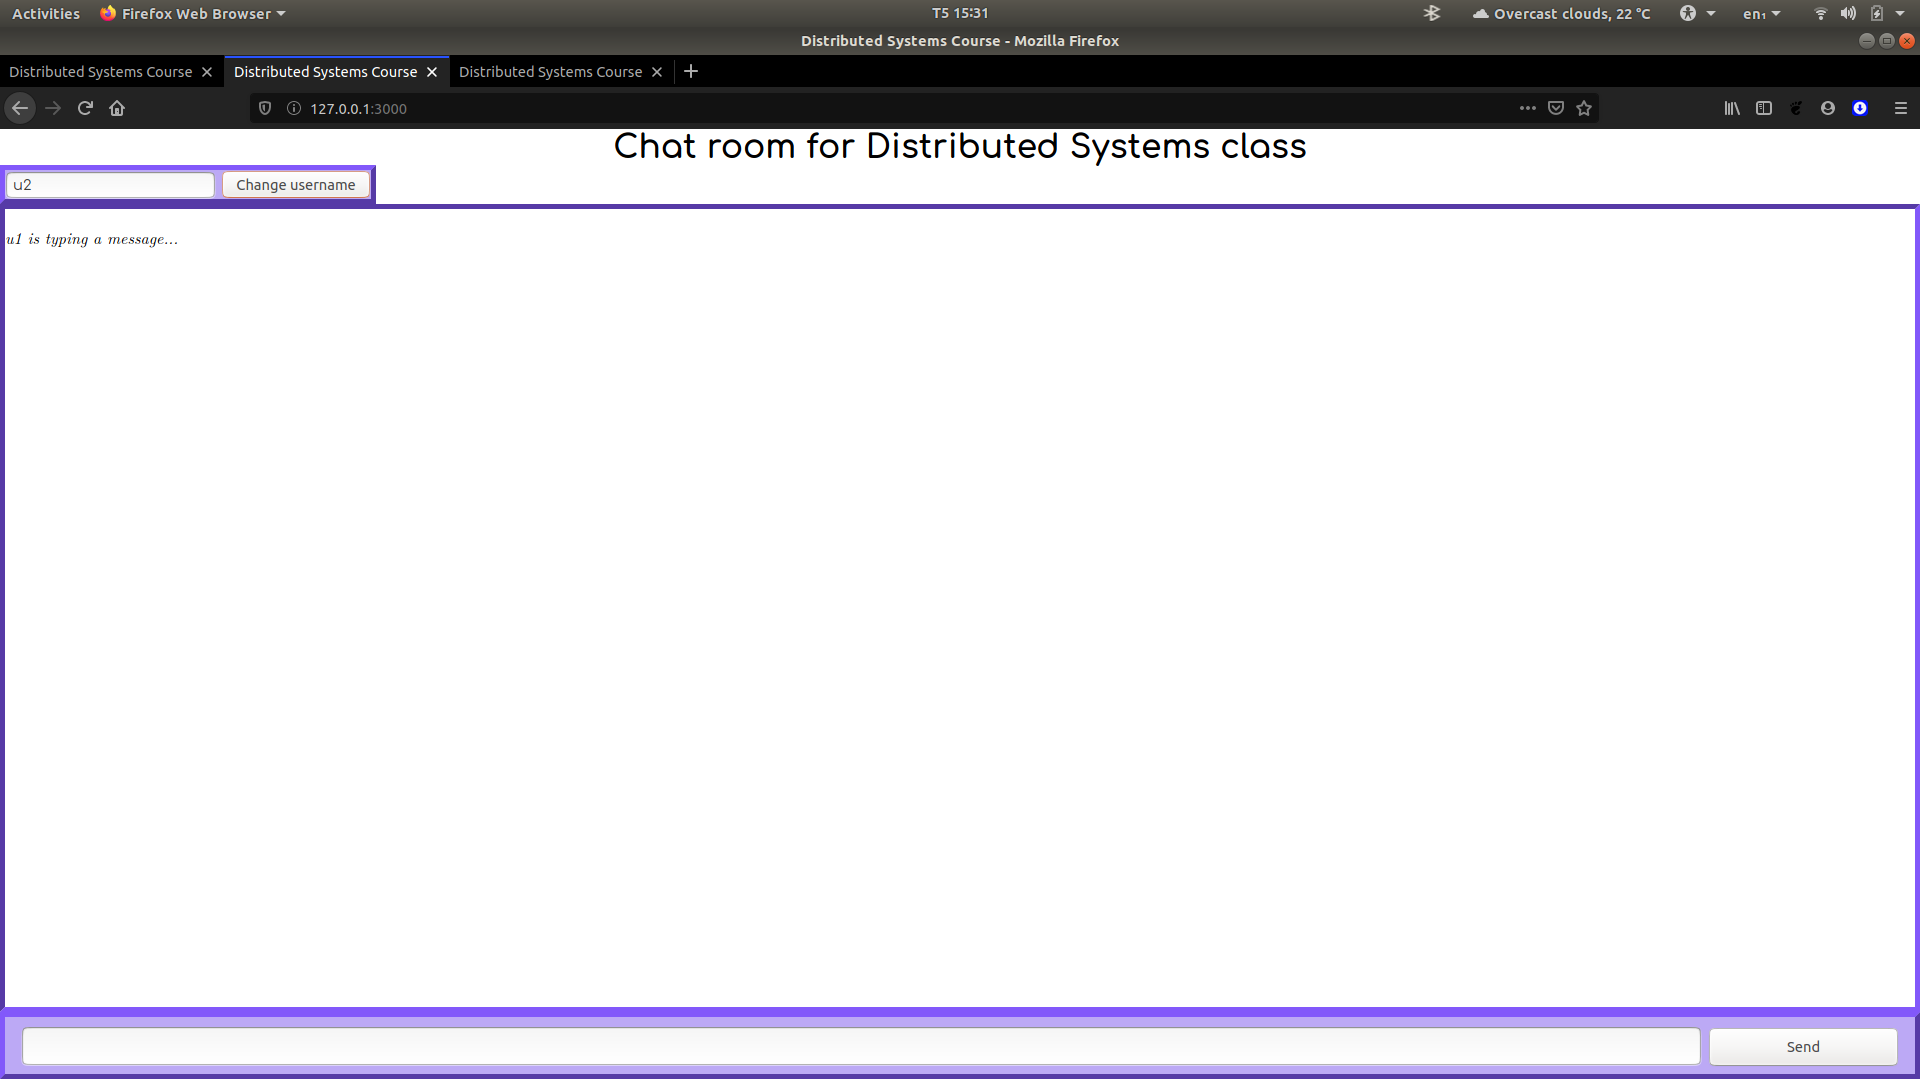
\includegraphics[width=\linewidth]{u2-notsend.png}
    		\caption{At the same time, on user u2's instance}
  		\end{subfigure}
  		\begin{subfigure}[b]{0.4\linewidth}
    		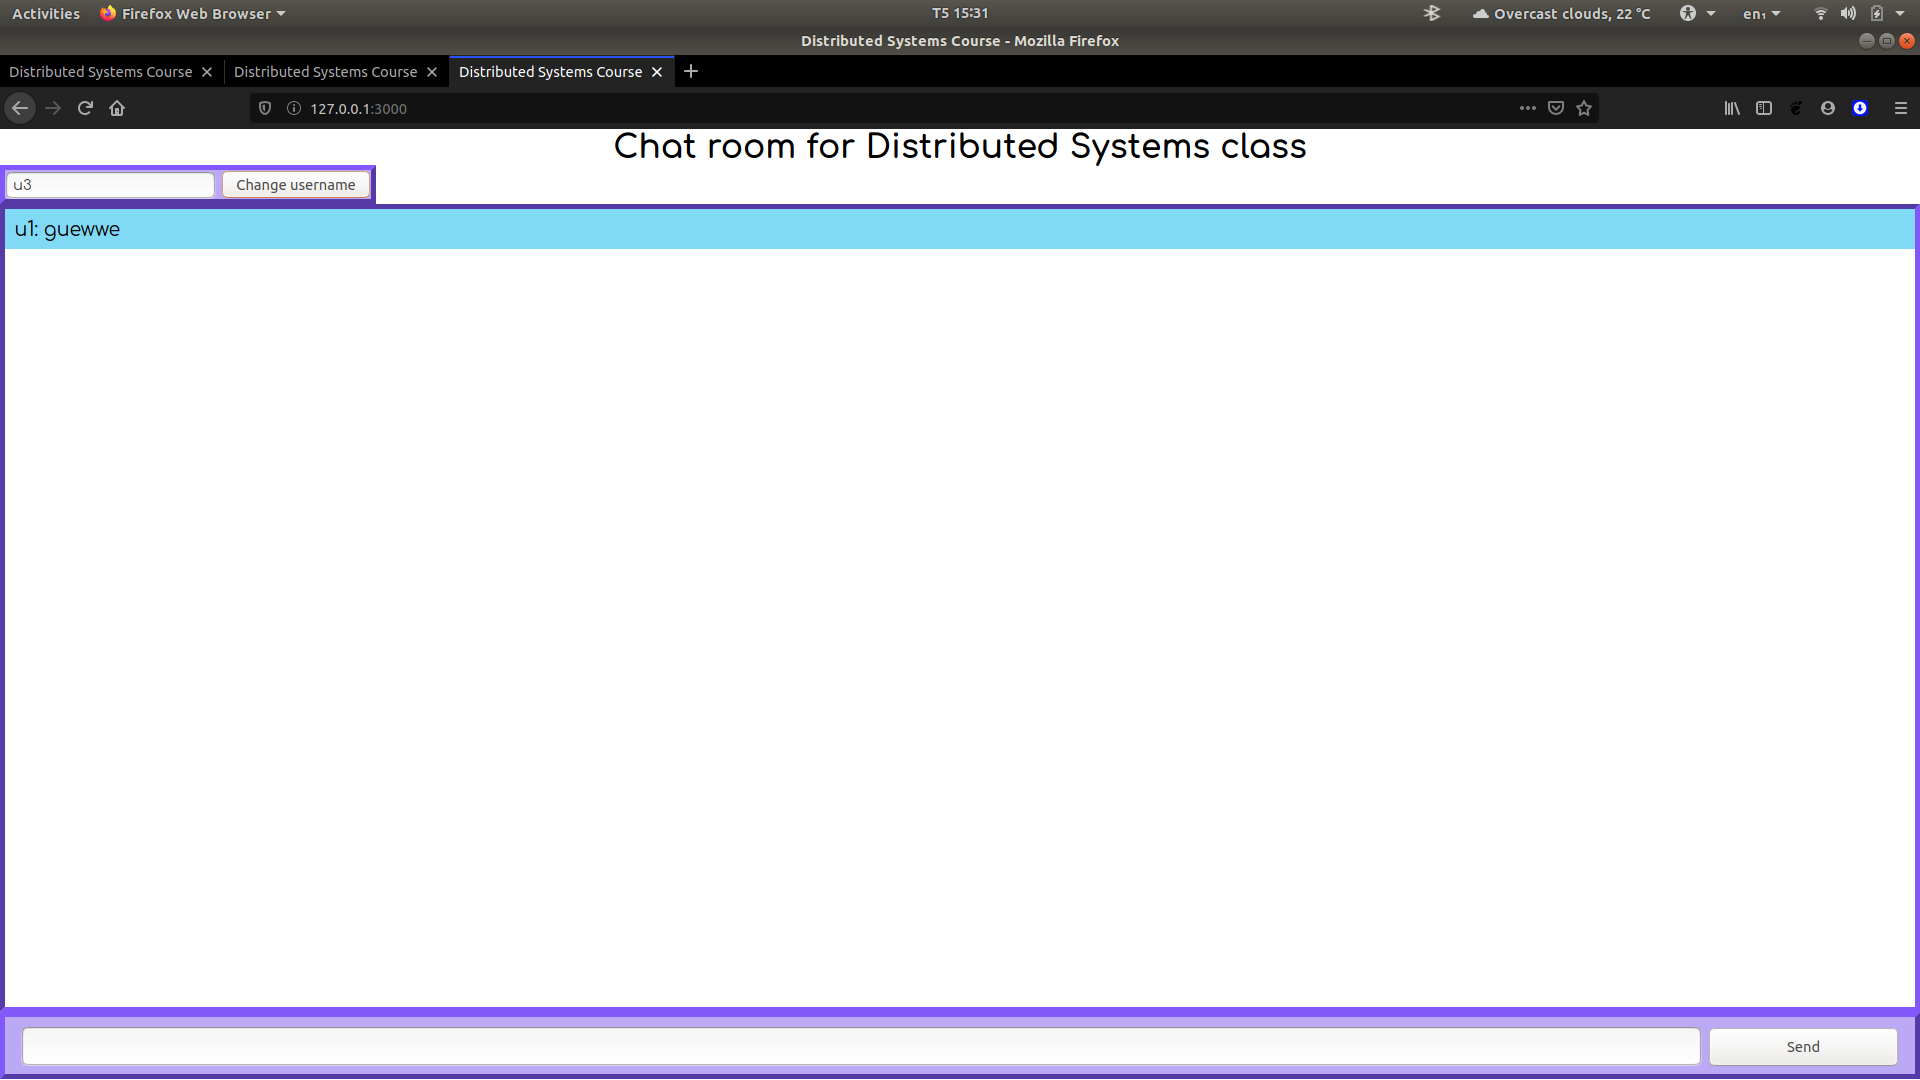
\includegraphics[width=\linewidth]{u3-aftersend.png}
    		\caption{After u1 hit send, on u3's instance}
  		\end{subfigure}
  		\caption{Final Product}
  		\label{fig:chat}
	\end{figure}
	
	\chapter{Chapter 4 Lab Work: Communication}
	\newpage
	\section{What is the code part that shows that the Server assigns the correlation ID to the response?}
  	\begin{figure}[h!]
  		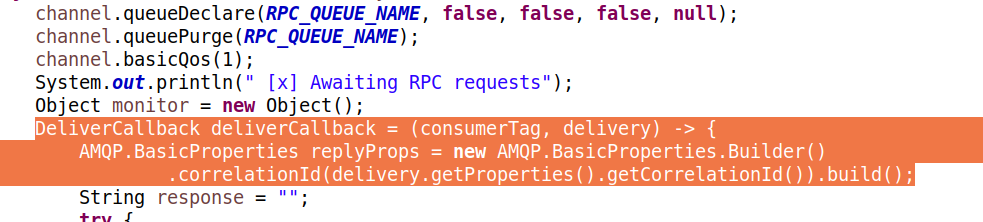
\includegraphics[width=\linewidth]{assign-corr-id.png}
  		\caption{Assigning correlation ID}
  		\label{fig:corr-id}
	\end{figure}
  	The part the Server assigns the correlation ID is highlighted in the figure \ref{fig:corr-id}
	
	\section{You base on both code of Client and Server program to explain which code shows that the Client sends request to Server through rpc\_queue and create a new queue to wait for the reply of the Server.}
	\begin{figure}[h!]
		\centering
  		\begin{subfigure}[b]{0.4\linewidth}
  		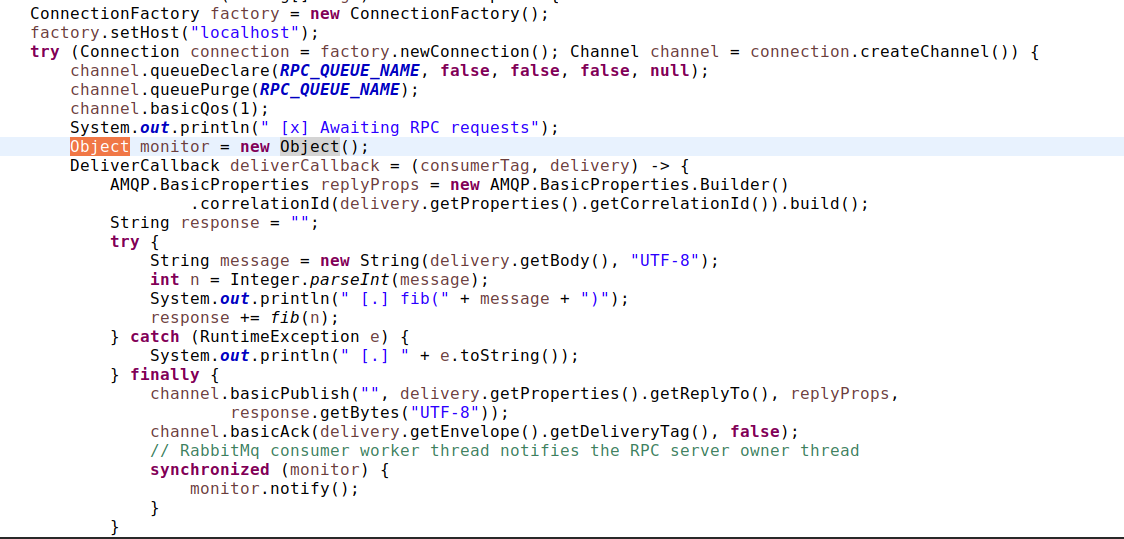
\includegraphics[width=\linewidth]{server-rpc-queue.png}
    		\caption{Receive request and response to request Server side}
  		\end{subfigure}
  		\begin{subfigure}[b]{0.4\linewidth}
    		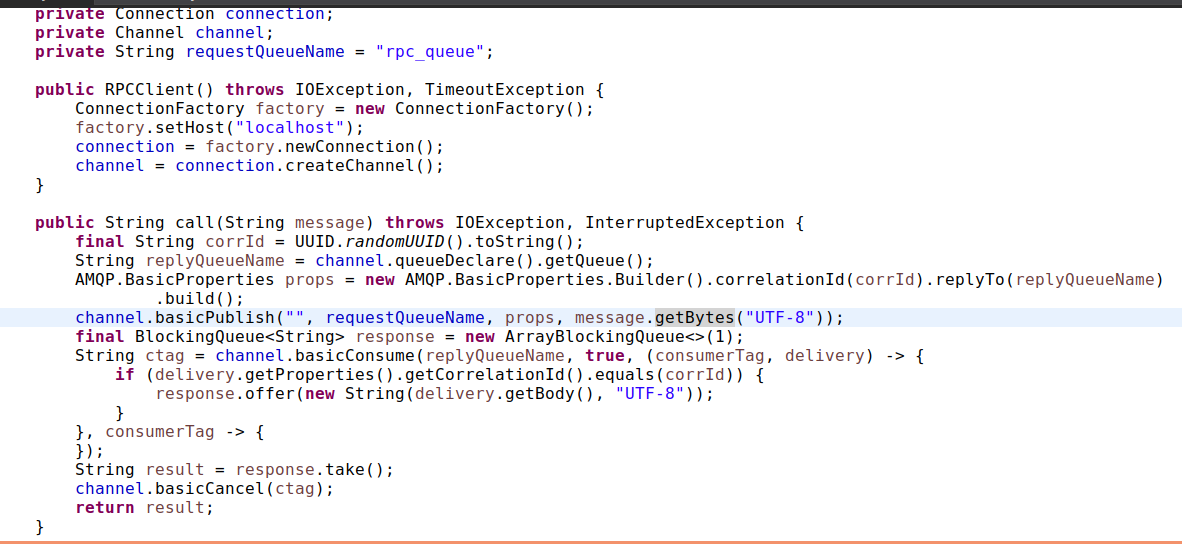
\includegraphics[width=\linewidth]{client-rpc-queue.png}
    		\caption{Sending request, create a new queue to wait the reply on Client side}
  		\end{subfigure}
  		\caption{Client sends request to Server through rpc\_queue}
  		\label{fig:rpc}
	\end{figure}
	
	\section{Try to add the delay to the Server program}
	The response from Server will be delayed thus making the Client waits for the response from previous request longer.\newpage
	\begin{figure}[t]
  		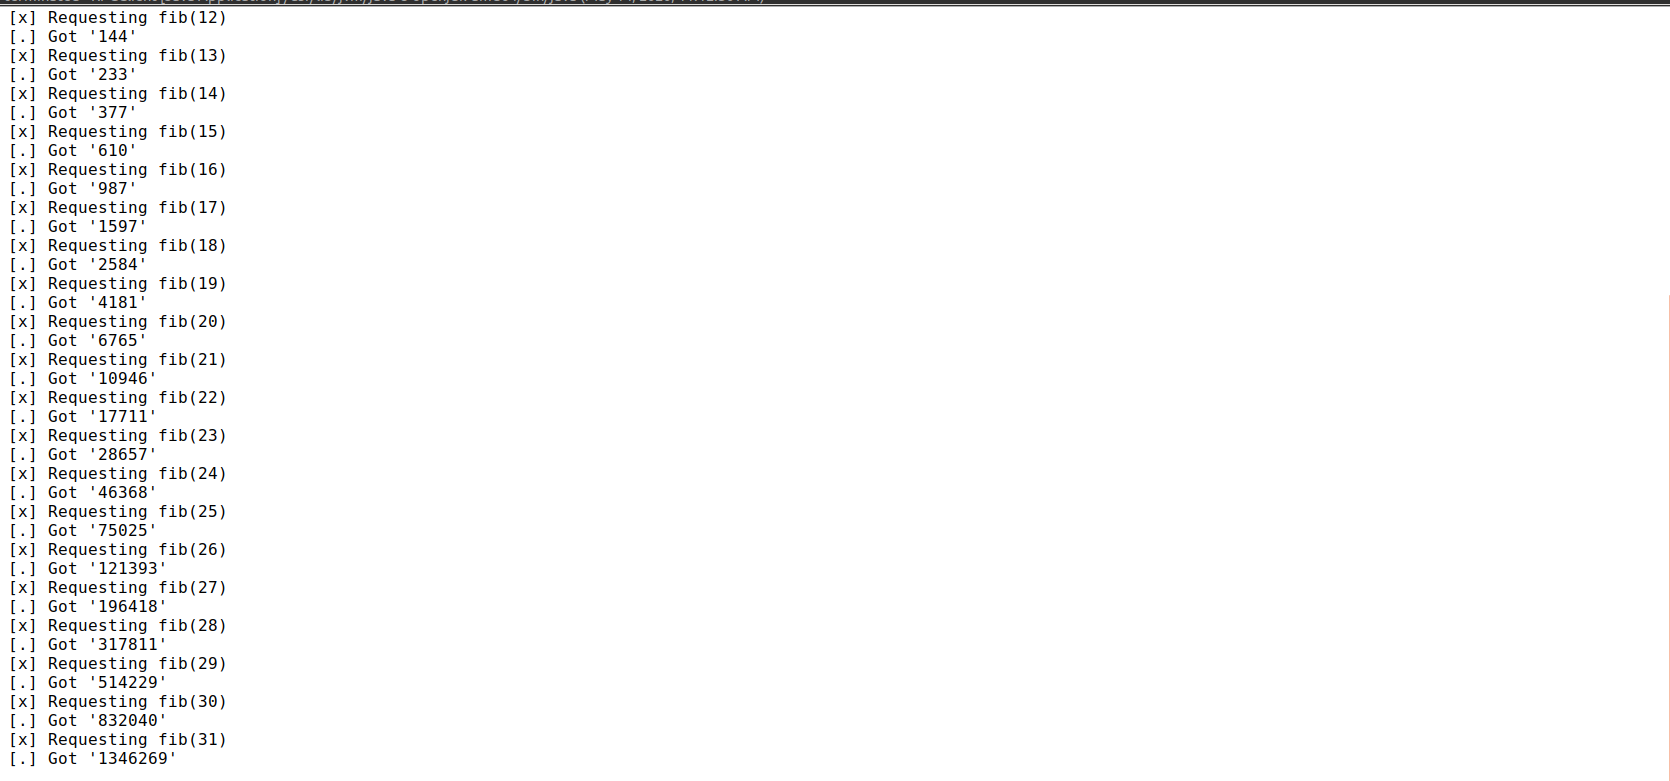
\includegraphics[width=\linewidth]{res-client.png}
  		\caption{Client Result}
  		\label{fig:res-client}
	\end{figure}
	When checking for queues, for n instances of Client are running, there are n queues for each instances plus the rpc\_queue. At all time, there are n-1 ready messages and 1 unacknowledged messages at rpc\_queue since the number on ArrayBlockingQueue equals to 1. The message on n unique queues for n instances will be transfered to rpc\_queue very fast thus it could be said that the ready messages and unacknowledged messages number equals to 0.
	\begin{figure}[h!]
		\centering
  		\begin{subfigure}[b]{0.4\linewidth}
  		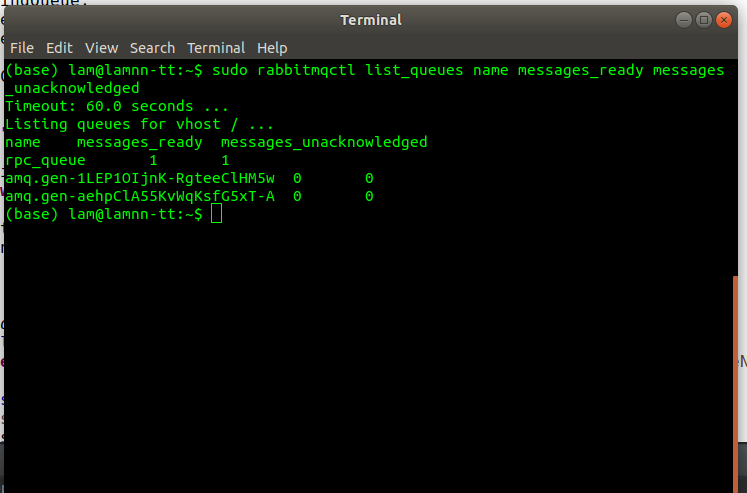
\includegraphics[width=\linewidth]{res-status.png}
    		\caption{When there are 2 instances of Client}
  		\end{subfigure}
  		\begin{subfigure}[b]{0.4\linewidth}
    		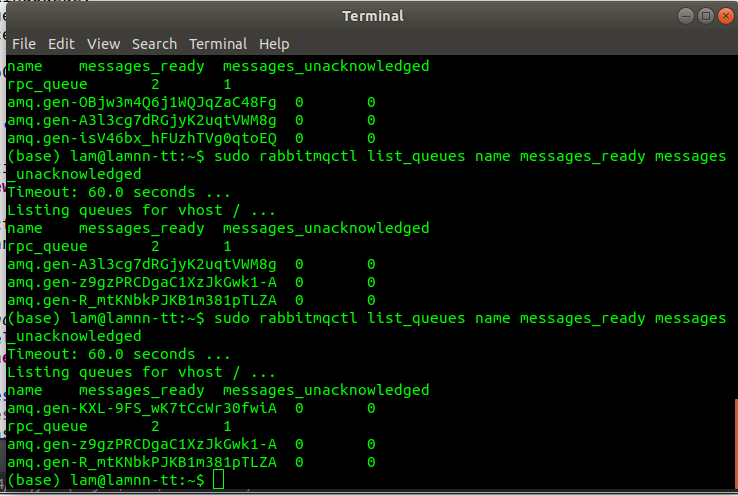
\includegraphics[width=\linewidth]{res-status-3.png}
    		\caption{When there are 3 instances of Client}
  		\end{subfigure}
  		\caption{Status of queues}
  		\label{fig:status}
	\end{figure}
	
	\section{Important note for the video streaming part.}
	\begin{enumerate}
		\item For this part, I will use my own laptop and my home computer connected over the home network.
	\end{enumerate}
	
	\section{What is the IP address of your 2 machines? How to ping each other?}
	The server will have the address: 192.168.0.109
	The client will have the address: 192.168.0.102
	\begin{figure}[h!]
		\centering
  		\begin{subfigure}[b]{0.4\linewidth}
  		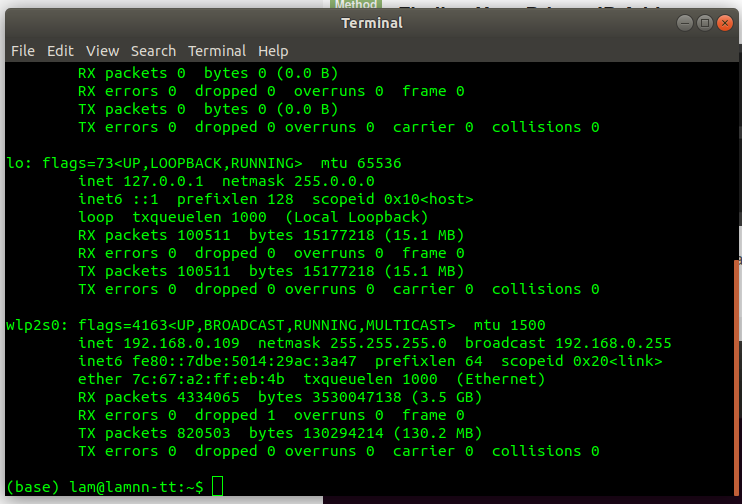
\includegraphics[width=\linewidth]{ip-server.png}
    		\caption{Of the Server}
  		\end{subfigure}
  		\begin{subfigure}[b]{0.4\linewidth}
    		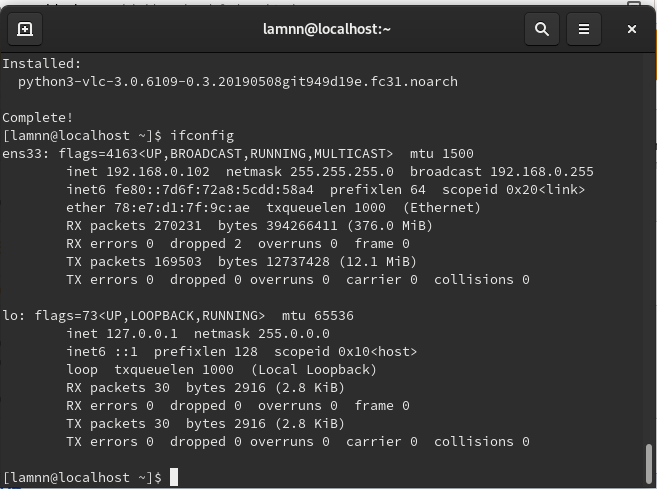
\includegraphics[width=\linewidth]{ip-client.png}
    		\caption{Of the Client}
  		\end{subfigure}
  		\caption{IP address}
  		\label{fig:addr}
	\end{figure}
	\\
	To ping each other we just use the standard ping function of Linux.
	\begin{figure}[h!]
  		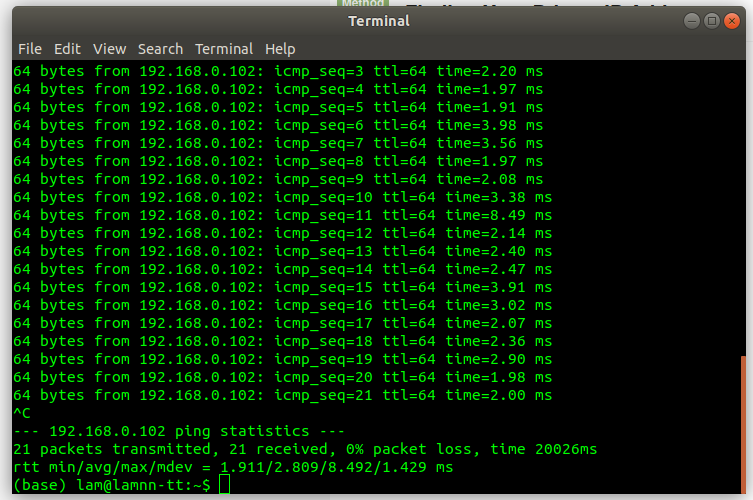
\includegraphics[width=\linewidth]{ping-to-client.png}
  		\caption{Ping from Server to Client}
  		\label{fig:ping}
	\end{figure}
	
	\section{Can you watch the video in the client machine? Evaluate the quality of the video streaming service.}
	When trying to connect to the server, we can see the video with good quality (no delay, no jitter, the stream is smooth)
	\begin{figure}[h!]
  		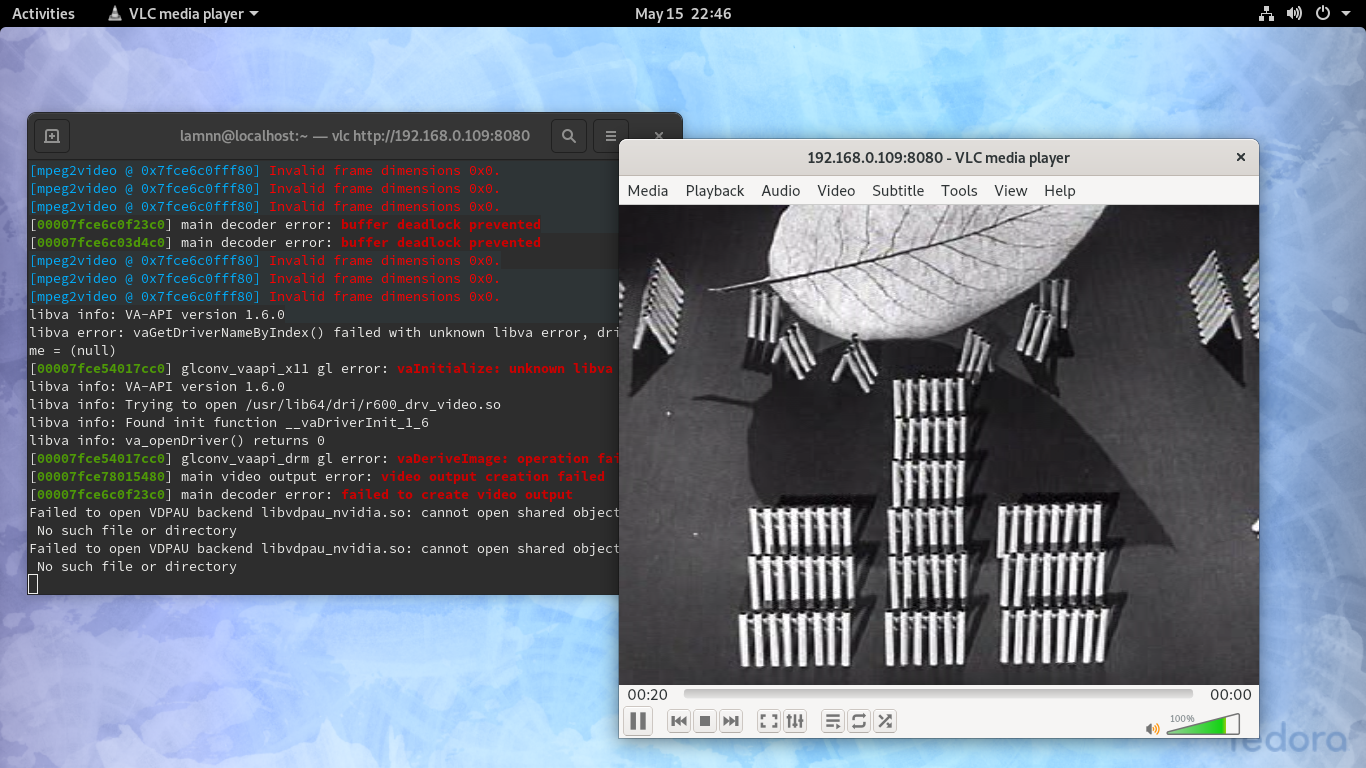
\includegraphics[width=\linewidth]{vid-perfect-cond.png}
  		\caption{Video streaming}
  		\label{fig:vid-p-cond}
	\end{figure}
	
	\section{What is the result of the ping test? Can you see an increase of 100 milliseconds?}
	\newpage
	\begin{figure}[h!]
  		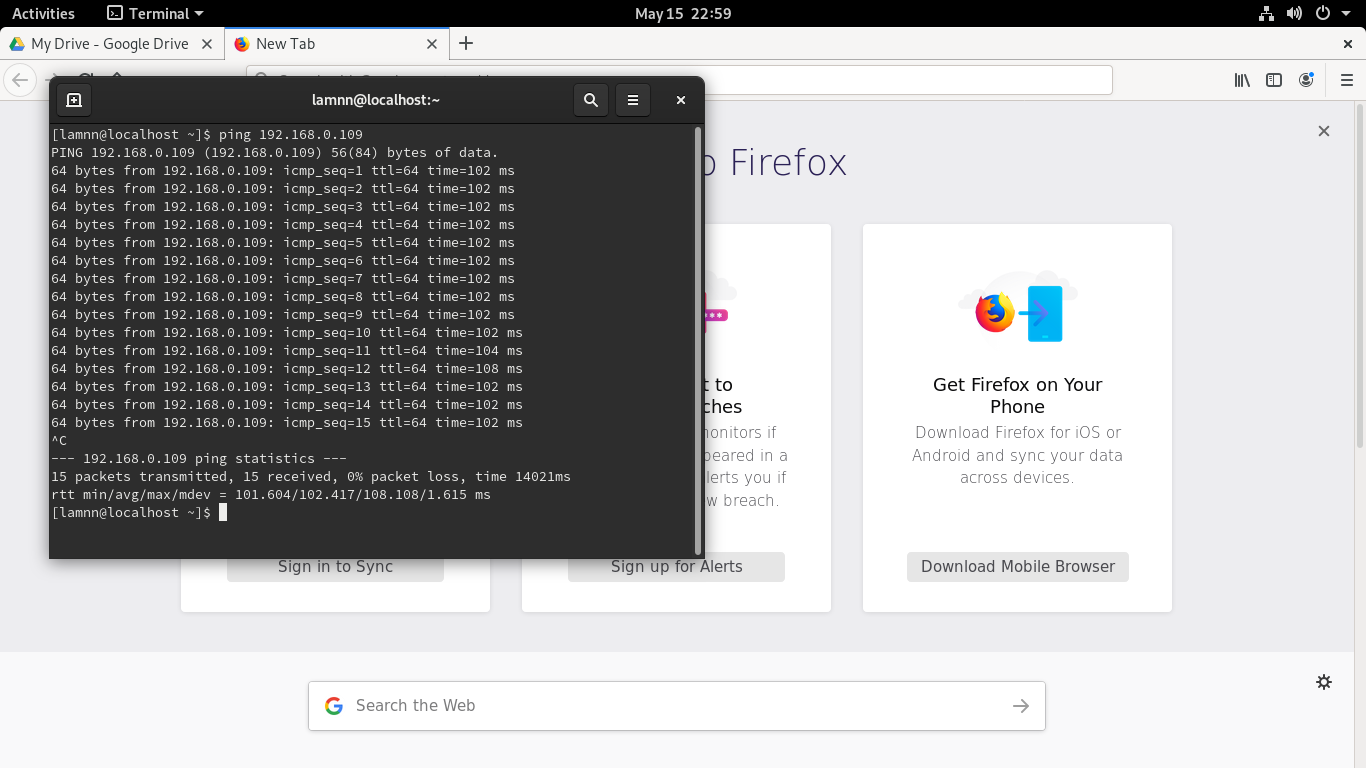
\includegraphics[width=\linewidth]{ping-delay-100.png}
  		\caption{Ping result when has delay=100ms}
  		\label{fig:ping-100}
	\end{figure}
	
	As figure \ref{fig:ping-100} shows, the time has been added 100ms from the previous time.
	
	\section{Disable the buffering function of VLC in Client machine. Then, evaluate the video quality at the Client machine. How can you conclude the impact of fix delay on video streaming service?}
	The frame periodically freezed. In conclusion, the impact of fix delay on video streaming service is constantly freeze the frames.
	
	\section{Evaluate the video quality atthe Client machine. How can you conclude the impact of delay variation on video streaming service?}
	The frame randomly freezed. In conclusion, the impact of delay variation on video streaming service is sometimes freeze the frames and for different duration.
	
	\section{Evaluate the video quality at the Client machine. How can you conclude the impact of fix loss rate on video streaming service? Try to increase the value of loss rate to see the impact more clear.}
	Sometimes, the video jumps from one scene to another scene without the transition. In conclusion, the impact of fix loss rate on video streaming service is the stream is periodically jitter. While it is annoying, if rate is low, it was bearable
	
	\section{Evaluate the video quality at the Client machine. How can you conclude the impact of loss rate variation on video streaming service? Try to increase this value to see the impact more clear.}
	There was a long duration of jitter. There was a 10 seconds black screen at some point.  In conclusion, the impact of loss rate variation on video streaming service is the stream is big gap in video. As a customer, this maybe unacceptable.
	
	\section{Evaluate the video quality at the Client machine. How can you conclude the impact of packet duplication on video streaming service? Try to increase this value to see the impact more clear.}
	There was a slight freeze at some frame.
	
	\section{Evaluate the video quality at the Client machine. How can you conclude the impact of packet corruption on video streaming service? }
	There is some frame that appeared after the frame that suppose to follow it. It makes the movement of the character seems to be backward.
	
	\chapter{Chapter 6 Lab Work: Synchronization}
	\newpage

\section{Launch this program several times. What do you notice? Explain it!}
There are some times when the program print out the wrong answer (expected 3000 every time, got less than 3000 at some instances)
\begin{figure}[h!]
	\centering
  	\begin{subfigure}[b]{0.4\linewidth}
  		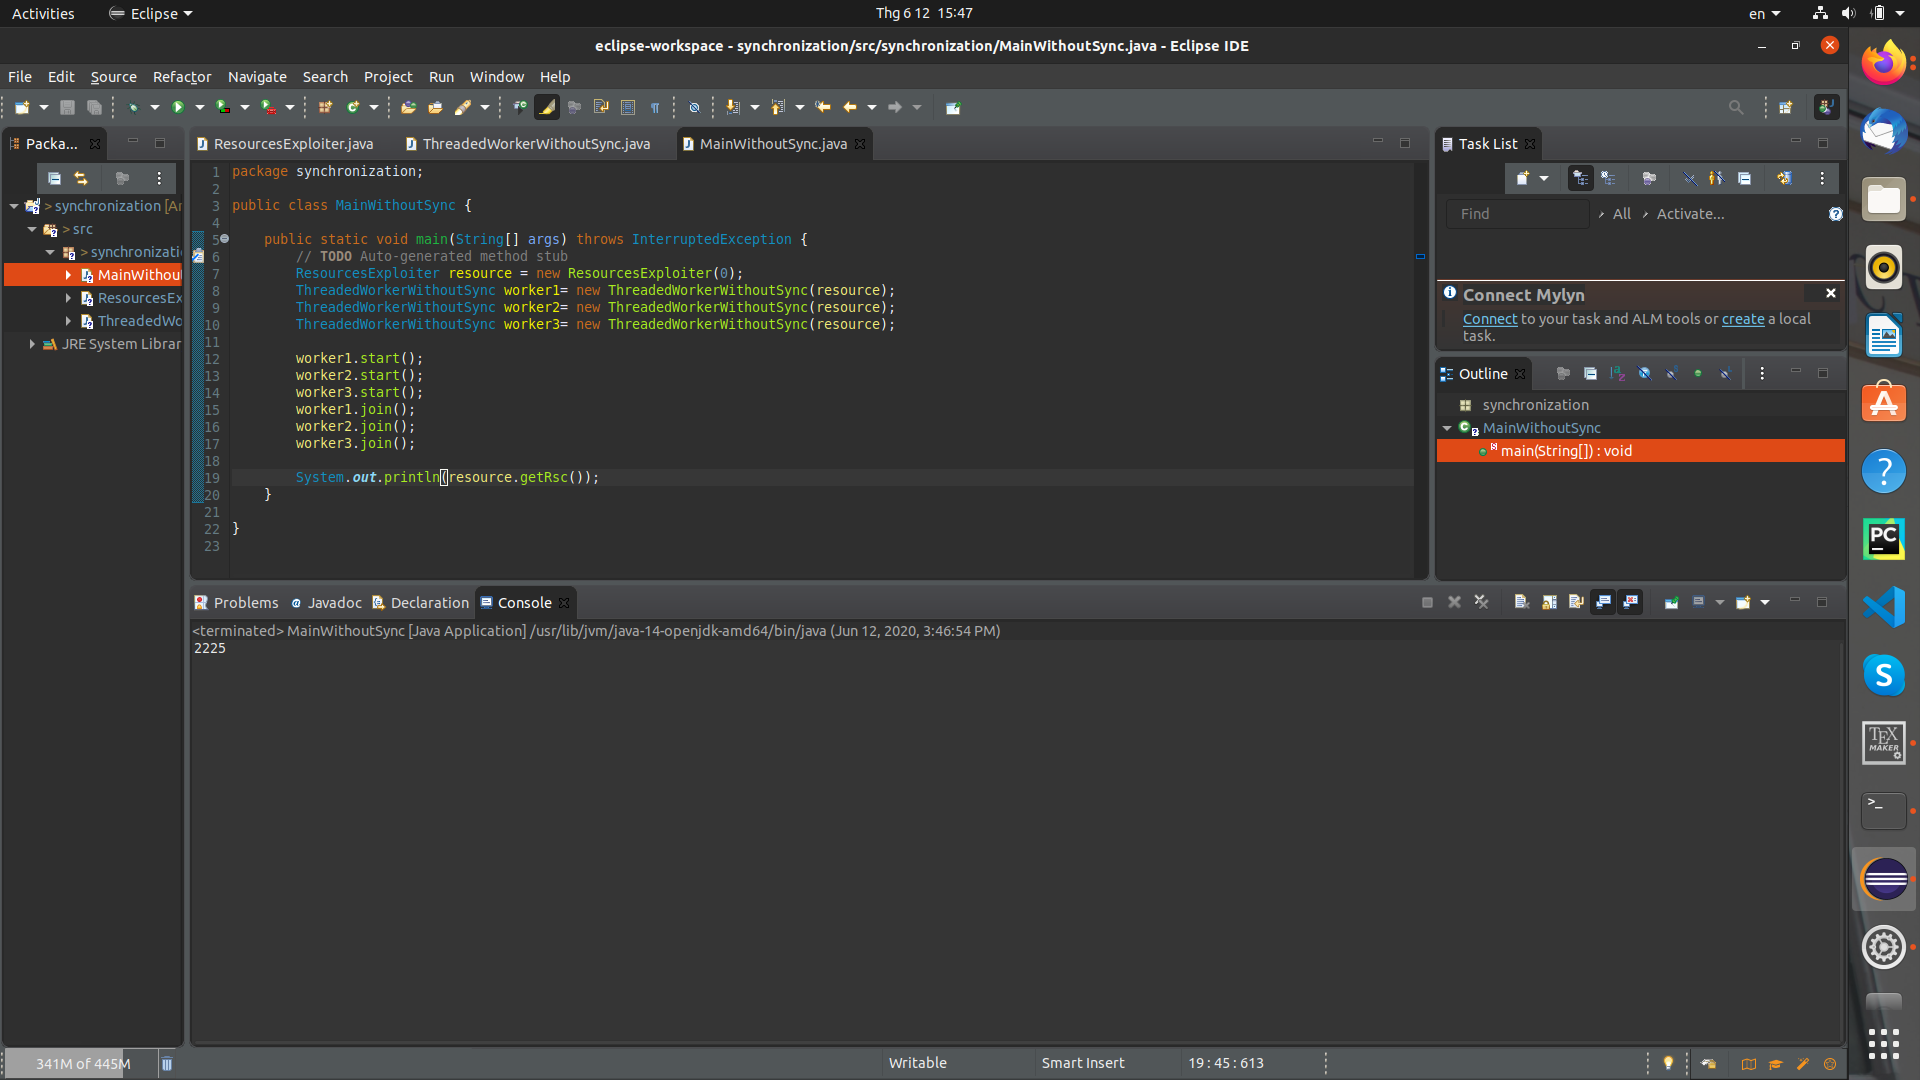
\includegraphics[width=\linewidth]{less-3000.png}
    	\caption{Unexpected result}
  	\end{subfigure}
  	\begin{subfigure}[b]{0.4\linewidth}
    	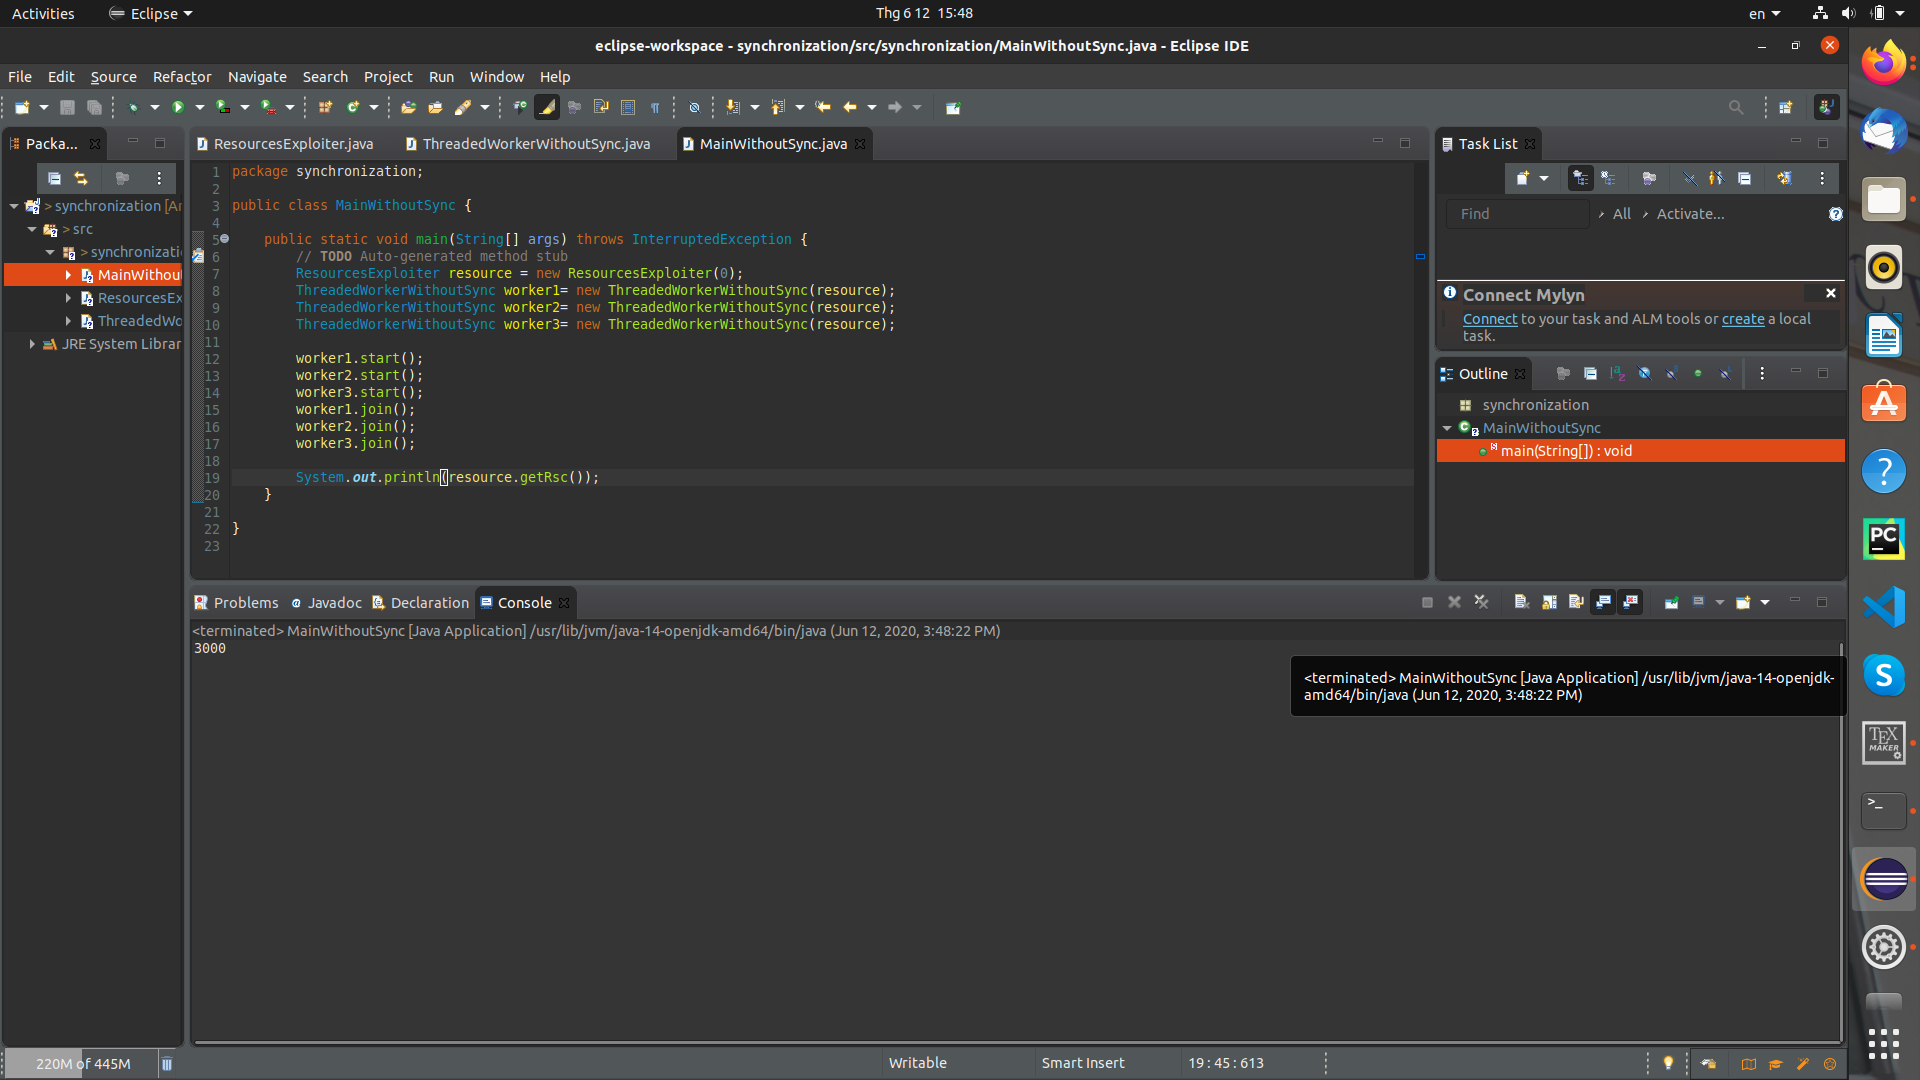
\includegraphics[width=\linewidth]{exact-3000.png}
    	\caption{The right result}
  	\end{subfigure}
  	\caption{Two types of result}
  	\label{fig:wosync}
\end{figure}
\\\textbf{Explanation:} Since there is not synchronization between each worker, sometimes two workers will try to access the resource at the same time. Each one, get the old value and add 1 to that and return the resource. Because of that, there are "less" addition happened and led to smaller result.
\section{Differences after synchronization. Explain}
The result is now consistently 3000 due to applying synchronization that makes workers access the resource in an "orderly" fashion.
\section{Differences after using lock. Explain}
The result is now consistently 3000 due to applying lock mechanism that makes only one worker can access the resource at one time.
\section{Complete this file above (in the part YOUR-CODE-HERE) with a loop to increase the variable shared by 1 for 5 seconds.}

\section{Try to increase the value of threads and the value of the constant NUM\_TRANS after each execution time until you obtain the different results between Balance and INIT\_BALANCE $+$ credits $-$ debits. Explain why do you get this difference.}
\begin{figure}[h!]
	\centering
  	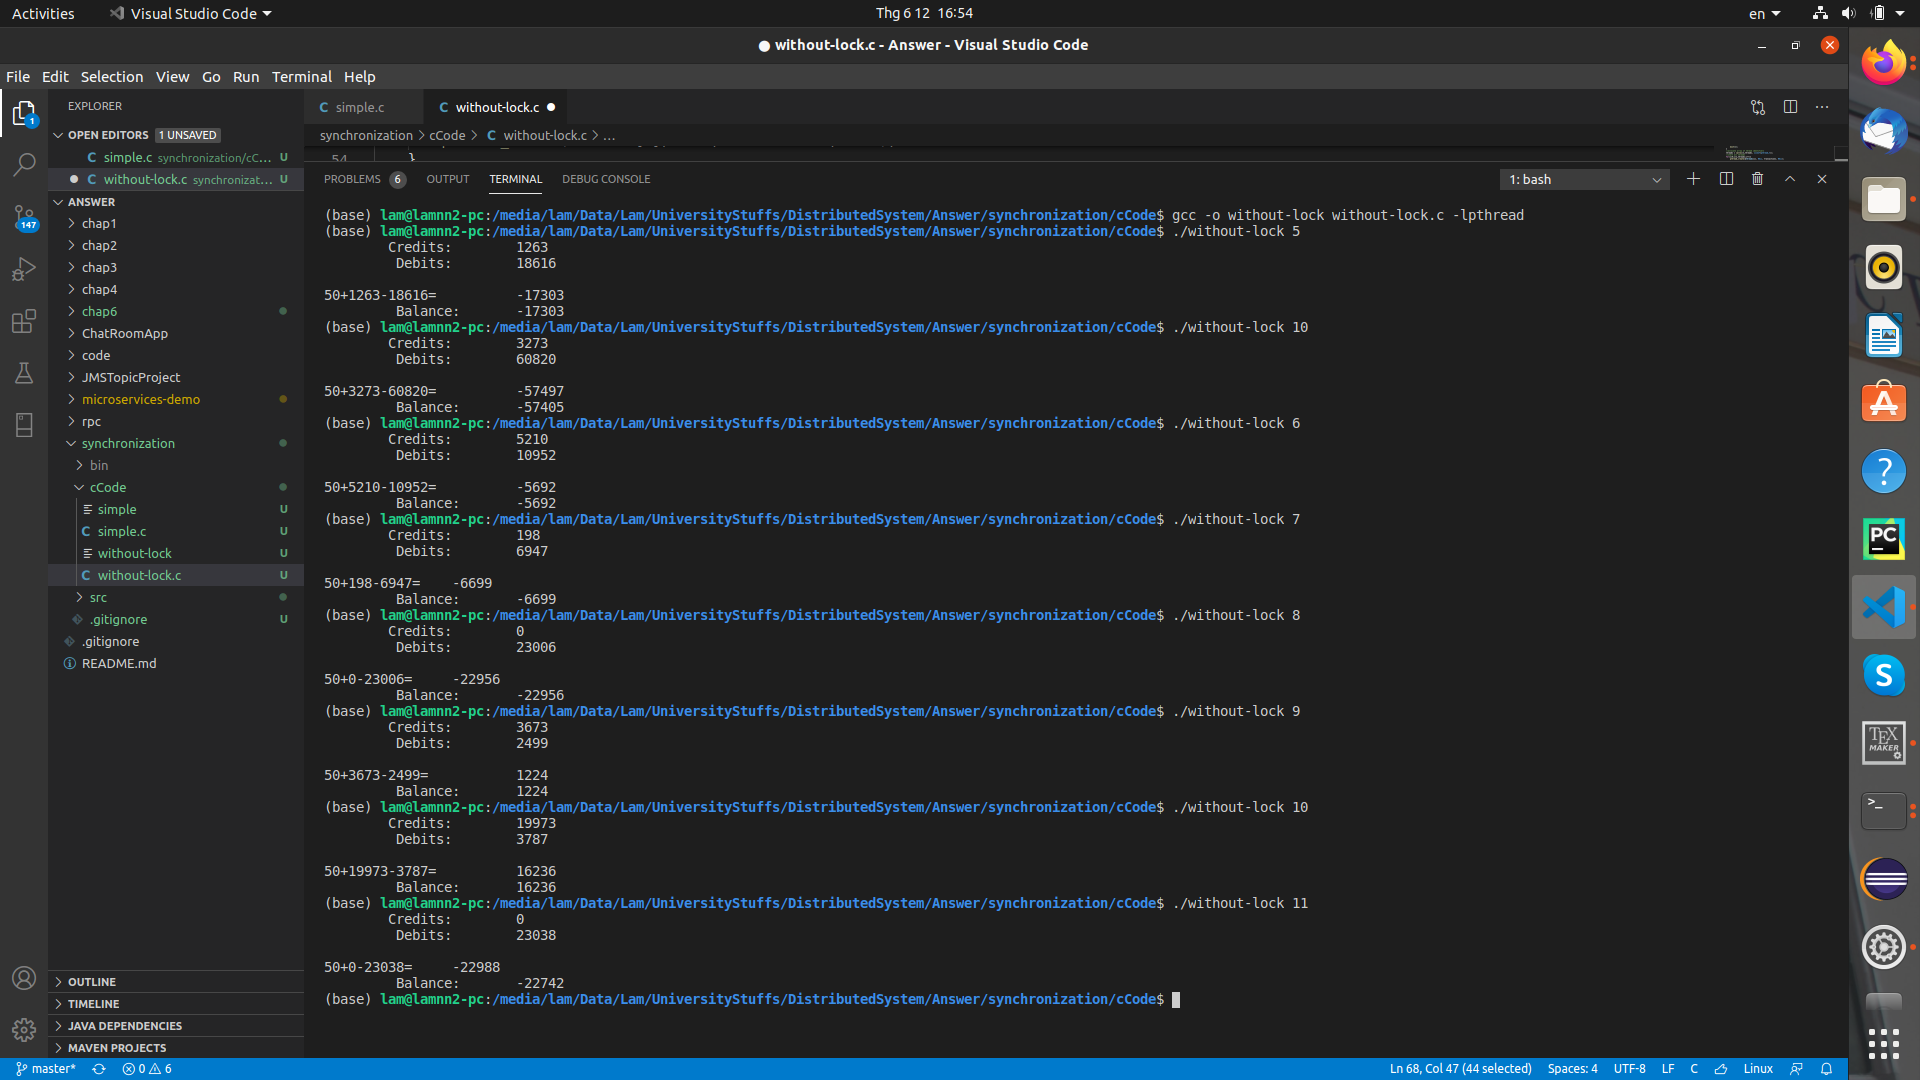
\includegraphics[width=\linewidth]{without-lock.png}
  	\caption{Result when there is not any lock}
  	\label{fig:wolock}
\end{figure}
Since every threads can access freely to the resource, when calculate the balance and there are more than one thread try to calculate that, it will not return the desired result (the whole operations of N thread involved) instead it updates the value according to the last to complete it operation. The higher the number of threads, the bigger chance of this to happened. The save option would be to make variable credits and debits exclusively used of each other and each thread only performs a credit or debit but not both.

\section{Try to build and run this program. Launch it repeatedly until you see the difference between Shared and Expect values. Analyze the source code to understand the problem that leads to this difference.}
\begin{figure}[h!]
	\centering
  	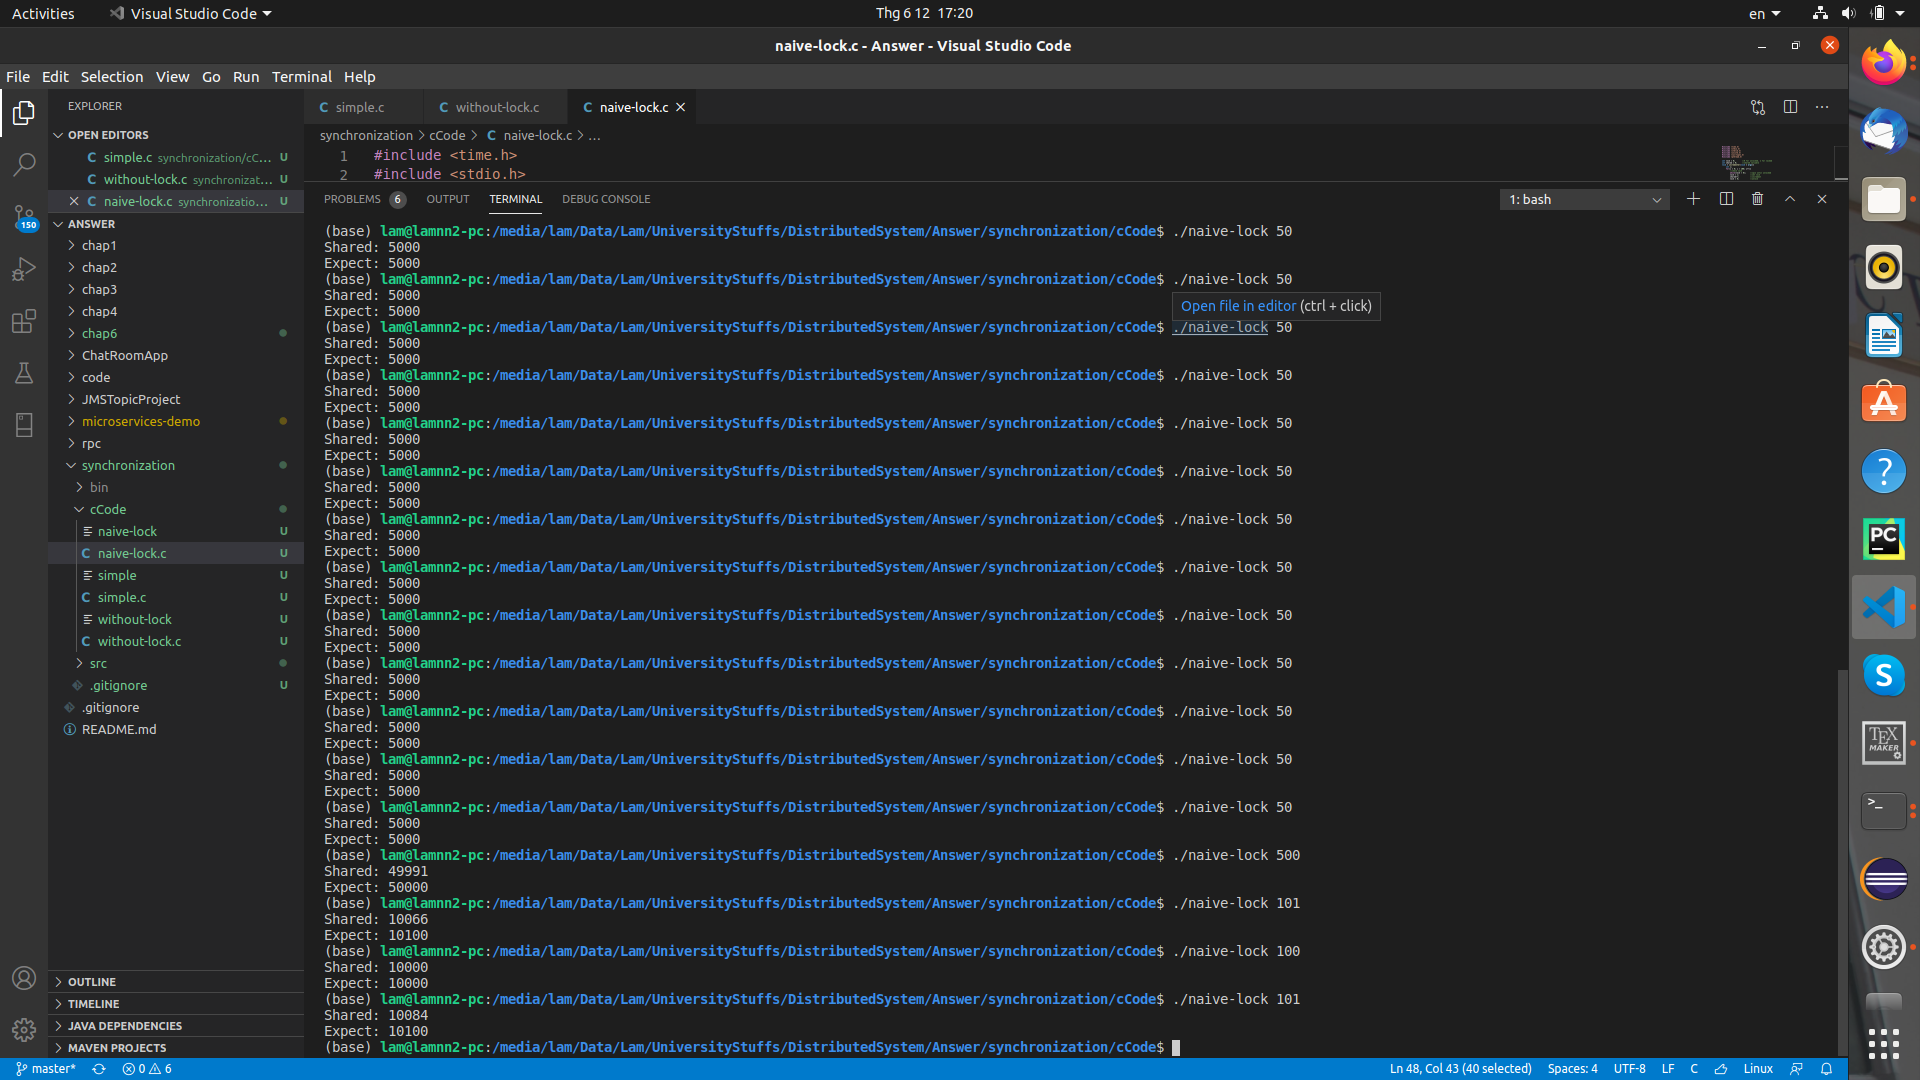
\includegraphics[width=\linewidth]{naive-lock.png}
  	\caption{Result when using naive lock}
  	\label{fig:naivelock}
\end{figure}
Since naive lock can only work for when the number of thread is smaller than 100 (as declared in the increment function), if the number of threads is larger than 100, it will immediately have a problem.

\section{What is the improvement after using mutex lock}
When use mutex lock, I saw that the number of error reduced dramatically. The error rate is nearly zero (out of all the time I run the program it return the different answer once). 

\section{Compare the run times of the two strategies to prove that Fine Locking is faster and much faster on larger load sets}
On 10000 threads, Coarse Locking runs in about 3 seconds. Meanwhile, Fine Locking runs in about 1.5 seconds.

\section{Run this program and what do you get as output? Explain what the deadlock is}
The program will forever runs and it never give the output.\\
Deadlock: deadlock is a state in which each member of a group is waiting for another member, including itself, to take action, such as sending a message or more commonly releasing a lock. In this particular problem, fun\_1 gets the lock of resource a first while fun\_2 gets the lock of resource b. 2 processes need both lock to work, but since neither can acquire the pair of locks so they will forever wait each other.
\end{document}